%%% TeX-command-extra-options: "-shell-escape"
%!TEX options=--shell-escape

%----------------------------------------------------------------------------------------
%   PACKAGES AND THEMES
%----------------------------------------------------------------------------------------
\documentclass[aspectratio=169,xcolor=dvipsnames]{beamer}
% \usetheme{Simple}

\usepackage{pgfpages}

%\setbeameroption{show notes}
\setbeameroption{show notes on second screen}
\setbeamertemplate{note page}[plain]

\usepackage{hyperref}
\usepackage{graphicx} % Allows including images
\usepackage{booktabs} % Allows the use of \toprule, \midrule and \bottomrule in tables
\usepackage{nicefrac}

% hyperlinks
\usepackage{hyperref}
\hypersetup{
    colorlinks=true,
    linkcolor=, % no color for internal links
    filecolor=magenta,
    urlcolor=blue,
}

% code
% \usepackage{minted}
% \setminted{
%     fontsize=\footnotesize,
%     autogobble,
%     bgcolor=mygray,
%     fontsize=\small
% }

% colors
\usepackage{xcolor}
\definecolor{mygray}{gray}{0.95} % define color - grey scale: 0=dark - 1=light

% packages added with respect to overleaf
\usepackage[utf8]{inputenc}
\usepackage{lmodern}
\usepackage{textcomp}
\usepackage[most]{tcolorbox} % colored boxes

% custom commands
\definecolor{darkred}{HTML}{CC0000}
\newcommand\textveryimp[1]{\textcolor{darkred}{\underline{\textbf{#1}}}} % text bold+red+underlined
\newcommand\textimp[1]{\underline{\textbf{#1}}} % text bold+red+underlined
\newcommand\textcode[1]{\textcolor{gray}{\texttt{#1}}} % text typewriter font + gray

\newcommand\blfootnote[1]{%
  \begingroup
  \renewcommand\thefootnote{}\footnote{#1}%
  \addtocounter{footnote}{-1}%
  \endgroup
}

% figures
\usepackage{tikz}
% \usetikzlibrary{shapes,backgrounds}
\usepackage{animate}
%\usepackage{media9}
% equations
\usepackage{amsmath}
\usepackage{amssymb}
\usepackage{empheq}
\usepackage{makecell}

% images
\graphicspath{ {./images/} } % Relative path to image directory

% insert table of content before each section
% \AtBeginSection[]
% {
%     \begin{frame}
%         \frametitle{Table of Contents}
%         % \tableofcontents[currentsection]
%     \end{frame}
% }
% \setbeamertemplate{subsection in toc}[subsections numbered] % add numbers in front of subsections
% \setbeamertemplate{subsection in toc}{\leavevmode\leftskip=2em$\bullet$\hskip1em\inserttocsubsection\par} % add bullets in front of subsections
%\setbeamertemplate{subsection in toc}{\leavevmode\leftskip=3.2em\rlap{\hskip-2em\inserttocsectionnumber.\inserttocsubsectionnumber}\inserttocsubsection\par}
\setbeamertemplate{subsection in toc}{\leavevmode\leftskip=3.5em\rlap{\hskip-1.25em\inserttocsubsectionnumber.}\inserttocsubsection\par} % add indented subsection number

\setbeamerfont{frametitle}{size=\scriptsize} % Set slide title fontsize
\setbeamercovered{transparent} % Set text to be semi-transparent during sequential overlay


%----------------------------------------------------------------------------------------
%   TITLE PAGE
%----------------------------------------------------------------------------------------

\title[short title]{Un- and Self-Supervised Learning}
\subtitle{Lecture 13}
\author{Automatic Image Analysis}
\titlegraphic{
  
\includegraphics[height=3cm]{cvlogo}
  
\includegraphics[height=3cm]{tublogo}
}
%\date{2021-04-23}

%----------------------------------------------------------------------------------------
%   PRESENTATION SLIDES
%----------------------------------------------------------------------------------------

\begin{document}

\begin{frame}
    \titlepage
\end{frame}

\begin{frame}{Why do machine learning?}
  \begin{figure}
    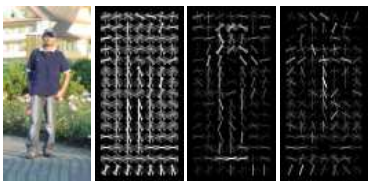
\includegraphics[width=0.8\textwidth]{hog}
  \end{figure}


  \note{
    \begin{itemize}
      \item How to connect our features to actual categories or measurements of image content in human terms?
      \item It would be hard to write heuristics to describe which HOG/SIFT feature corresponds to a dog or cat.
      \item There are two reason to make this connection.
            One is prediction of responses for unseen data.
            The other to analyze the connection between $x$ and $y$ (in statistics called inference).
      \item Image from Histograms of oriented gradients for human detection, Dalal \& Triggs
    \end{itemize}
  }
\end{frame}


\begin{frame}{What is machine learning?}

  \begin{figure}
    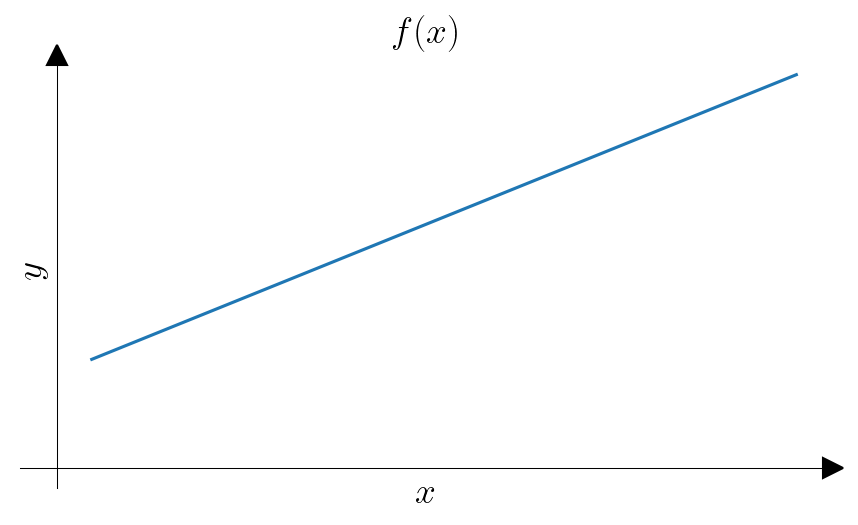
\includegraphics[width=0.8\textwidth]{ftrue}
  \end{figure}

  \note{
    \begin{itemize}
      \item We assume that there is a true mapping $f$ that maps from the image or feature space (predictor $x$) to e.g. an object category (response $y$).
      \item $x$ is also often called feature, input variable, just variable or independent variable.
      \item $y$ is also often called ground truth, target, label, output variable or dependent variable
      \item In the following we will often consider $x$ and $y$ to be multidimensional but visualize them mostly as scalars.
    \end{itemize}
  }
\end{frame}


\begin{frame}{What is machine learning?}

  \begin{figure}
    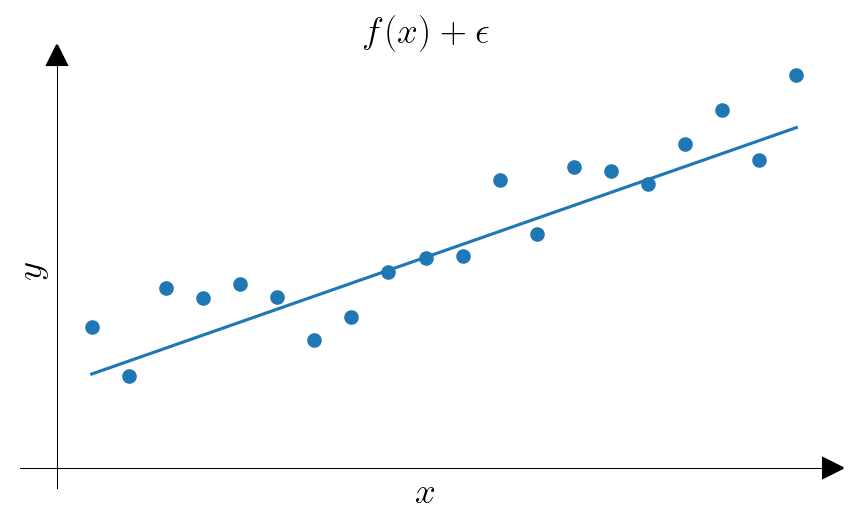
\includegraphics[width=0.8\textwidth]{feps}
  \end{figure}

\note{
  \begin{itemize}
    \item We want to estimate this function based on data we collected.
    \item When data is collected, we make an error $\epsilon$.
    \item This error is almost always of probabilistic nature. Our data is noisy.
    \item The set of measurements is denoted by $(Y, X)$ with all values collected for $X$ and their corresponding $y$s in $Y$.
  \end{itemize}
}
\end{frame}


\begin{frame}{Non-parametric Methods}

  \begin{figure}
    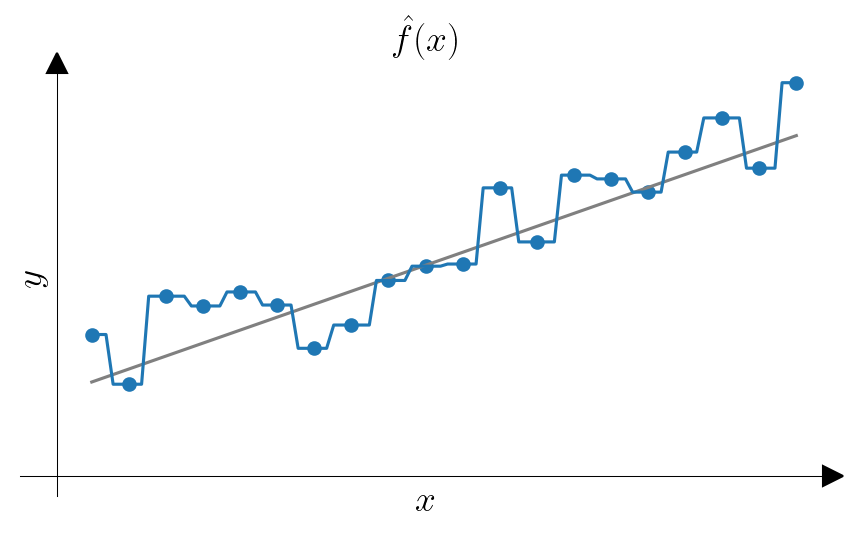
\includegraphics[width=0.8\textwidth]{fnoparam}
  \end{figure}
\note{
  \begin{itemize}
    \item Modeling of a wide range of functional forms possible.
    \item Usually very high number of observations necessary.
    \item In this case simply $\hat{f}(x) = Y_{argmin(|X-x|)}$
  \end{itemize}
}
\end{frame}


\begin{frame}{Parametric Methods}

  \begin{figure}
    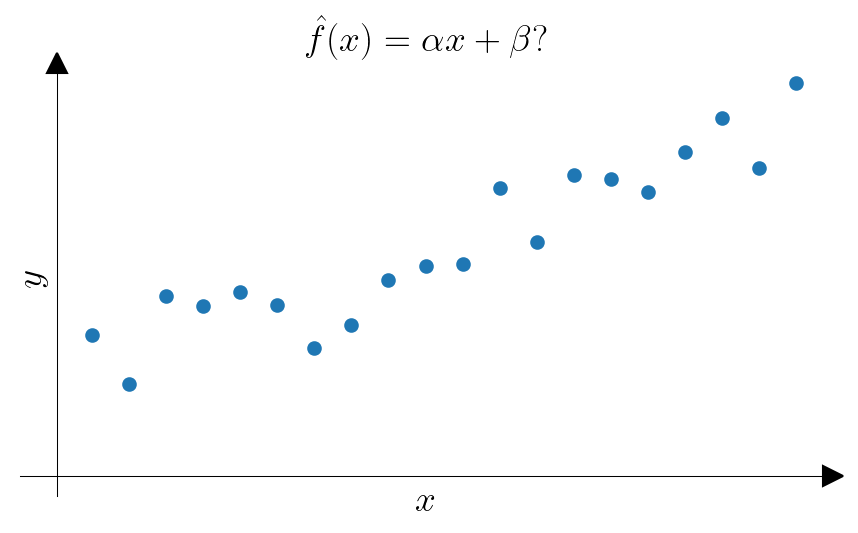
\includegraphics[width=0.8\textwidth]{fparam}
  \end{figure}
\note{
  \begin{itemize}
    \item We make an assumption about the functional form of $f$.
    \item In this case we might assume that the $f$ that generated our data is linear.
  \end{itemize}
}
\end{frame}


\begin{frame}{How can we estimate our parameters?}

  \vspace{1cm}
  \begin{equation*}
    E(\alpha, \beta) = \frac{1}{n}\sum_{i} (y_{i}-\hat{f}(x_{i}))^{2} = \frac{1}{n}\sum_{i} (y_{i}-\alpha x_{i} + \beta)^{2}
  \end{equation*}
\note{
  \begin{itemize}
    \item We need a criterion that tells us how well the estimation fits our data.
    \item An often used metric is the mean square error.
  \end{itemize}
}
\end{frame}

\begin{frame}{Linear Regression}

  \vspace{1cm}
  \begin{equation*}
    \frac{dE}{d\alpha} \stackrel{!}{=} 0 \text{ and } \frac{dE}{d\beta} \stackrel{!}{=} 0
  \end{equation*}
  \begin{align*}
    \hat{\alpha} & = \frac{\sum_{i}(x_{i}-\bar{x})(y_{i}-\bar{y})}{\sum_{i}(x_{i}-\bar{x})^{2}} \\
    \hat{\beta} & = \bar{y}-\hat{\alpha}\bar{x}
  \end{align*}
\note{
  \begin{itemize}
    \item To minimize the error, the first derivatives have to be zero.
    \item Using a linear model and mean square error allows for an analytical solution.
    \item Procedure is known as linear regression, a very simple and very popular method.
  \end{itemize}
}
\end{frame}


\begin{frame}
  \begin{figure}
    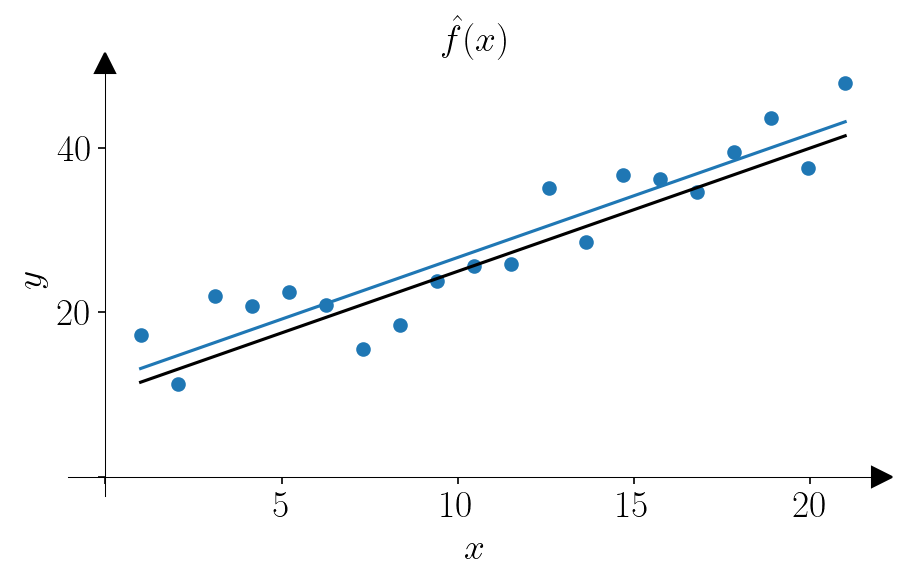
\includegraphics[width=0.8\textwidth]{linreg}
  \end{figure}
\note{
  \begin{itemize}
    \item Black shows the data generating ground truth, blue the estimate based on the measured data.
  \end{itemize}
}
\end{frame}


\begin{frame}{Error surface}

  \begin{figure}
    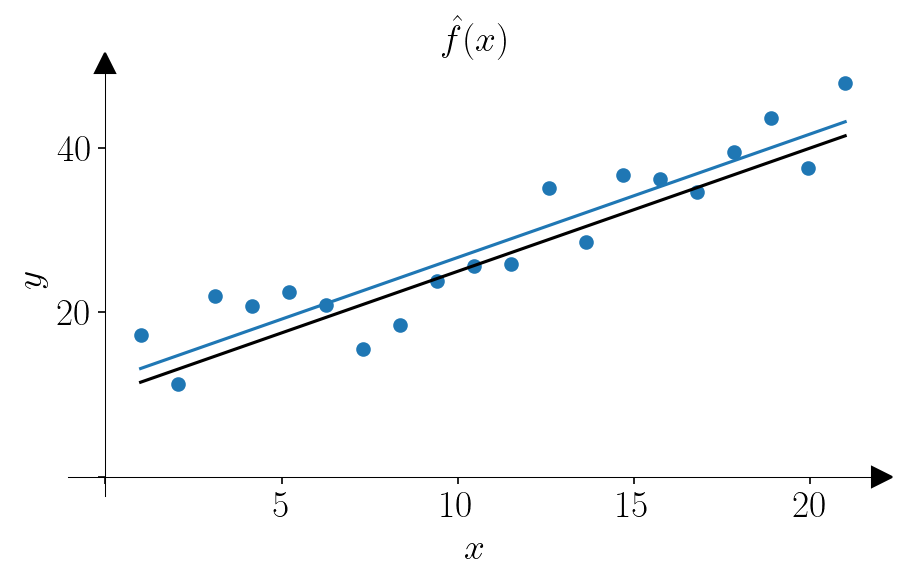
\includegraphics[width=0.4\textwidth]{linreg}
  \end{figure}
  \begin{figure}
    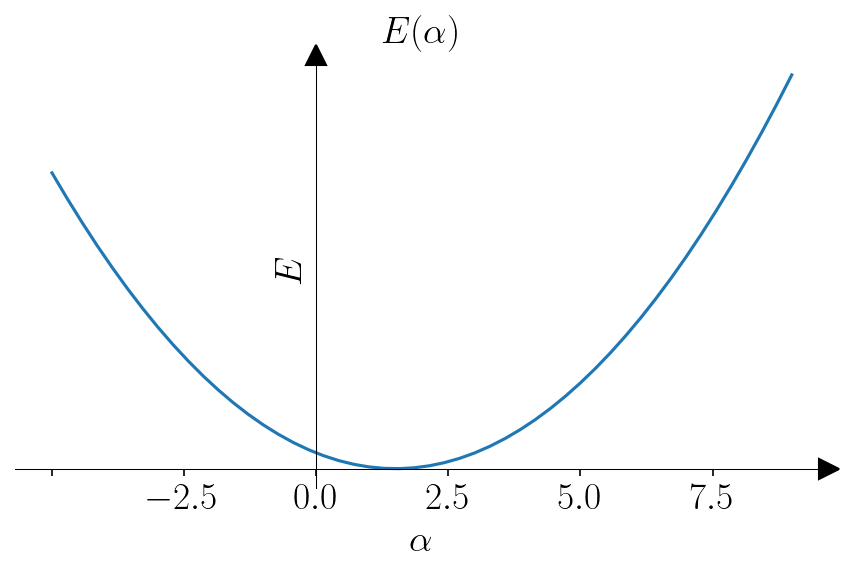
\includegraphics[width=0.4\textwidth]{erralpha}
    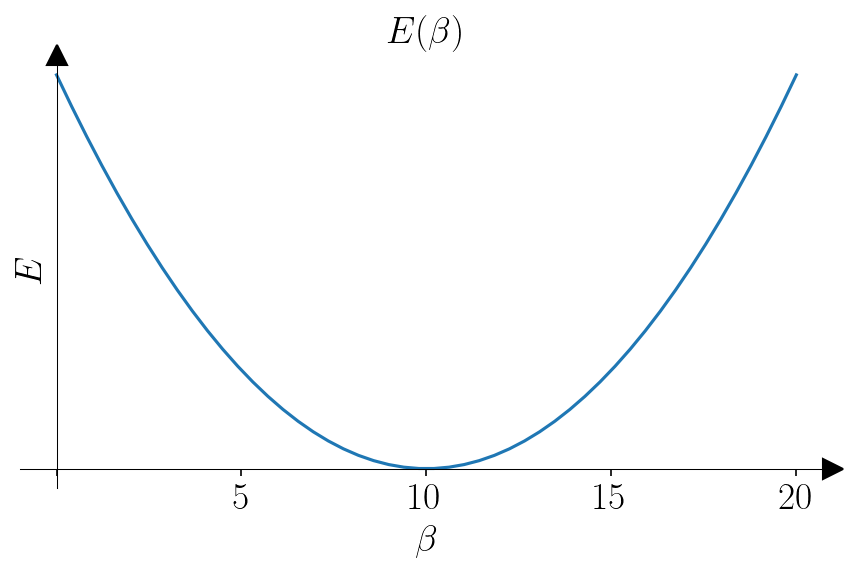
\includegraphics[width=0.4\textwidth]{errbeta}
  \end{figure}

\note{
  \begin{itemize}
    \item This slide shows the error surface of the linear model we just fitted to the data.
    \item On the left for the parameter alpha on the right for beta.
    \item We were lucky, not only has our problem a analytical solution it also has a convex error surface.
  \end{itemize}
}
\end{frame}


\begin{frame}{Error surface}

  \begin{figure}
    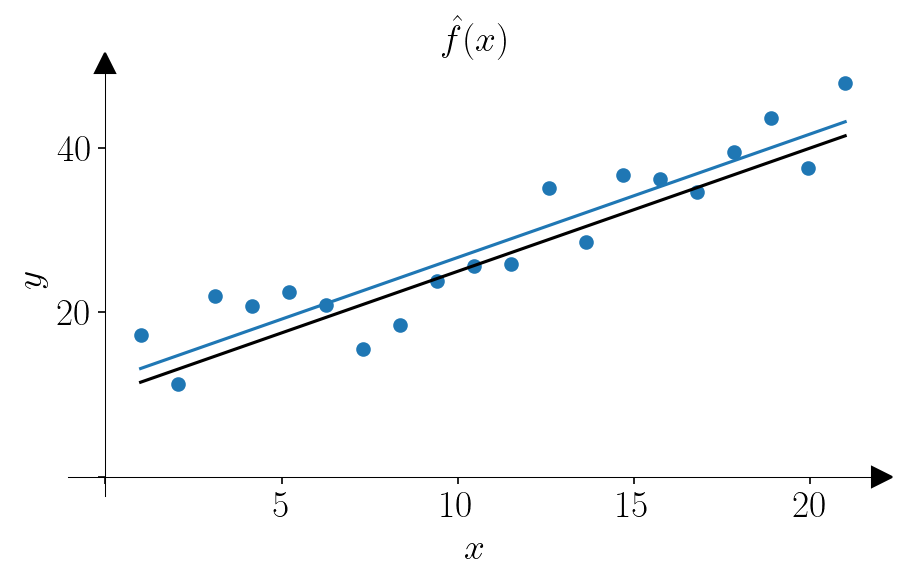
\includegraphics[width=0.4\textwidth]{linreg}
    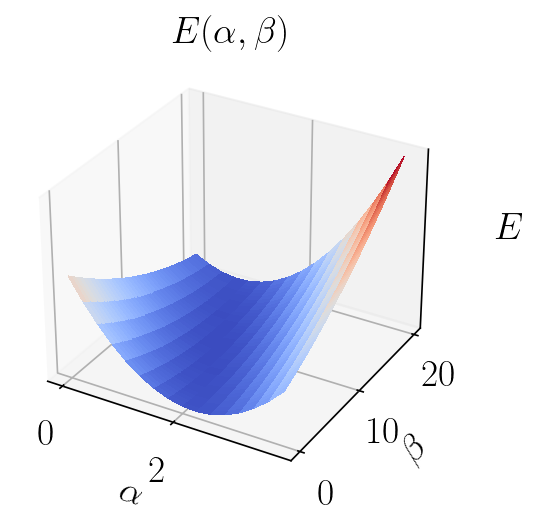
\includegraphics[width=0.4\textwidth]{err2d}
  \end{figure}

\note{
  \begin{itemize}
    \item Same function plotted in 2d.
    \item We were lucky, not only has our problem a analytical solution it also has a convex error surface.
  \end{itemize}
}
\end{frame}


\begin{frame}{Error surface}

  \begin{figure}
    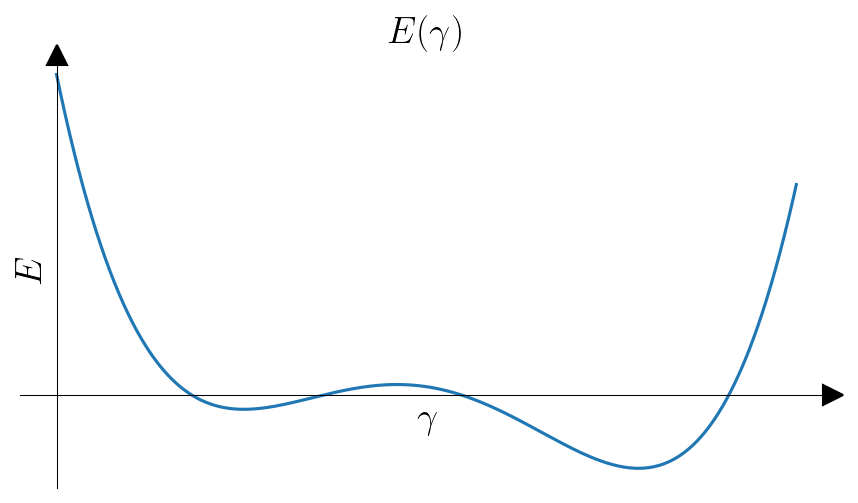
\includegraphics[width=0.8\textwidth]{nonconvex}
  \end{figure}

\note{
  \begin{itemize}
    \item Unfortunately, for more complex problems, this error surfaces are often non-convex.
    \item Especially when we can not find analytical solutions, local minima in such non-convex objective function can be problematic.
  \end{itemize}
}
\end{frame}


\begin{frame}{What if linear is not good enough?}

  \begin{figure}
    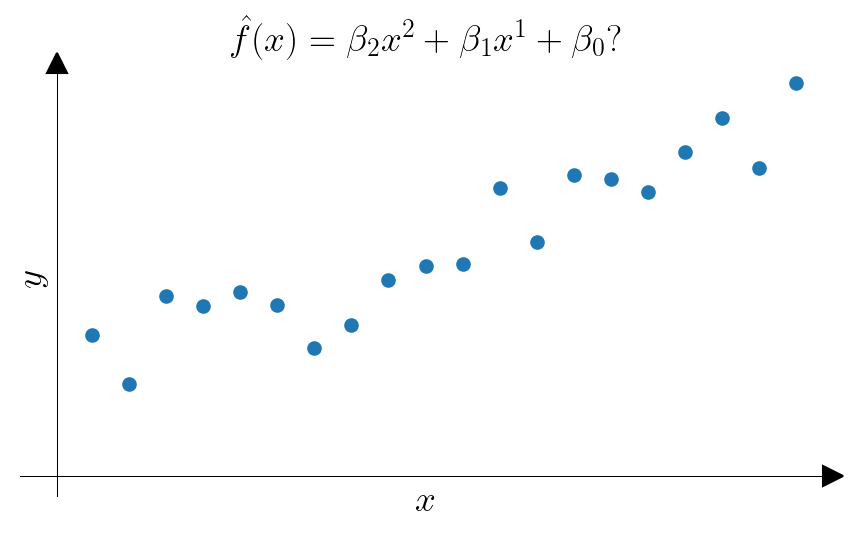
\includegraphics[width=0.8\textwidth]{fnonlin}
  \end{figure}
\note{
  \begin{itemize}
    \item A common pattern in machine learning is to apply linear methods trained on non-linear functions of the data.
    \item We map in a non-linear way to a higher dimensional features space and do linear regression.

  \end{itemize}
}
\end{frame}


\begin{frame}{What if linear is not good enough?}

  \begin{figure}
    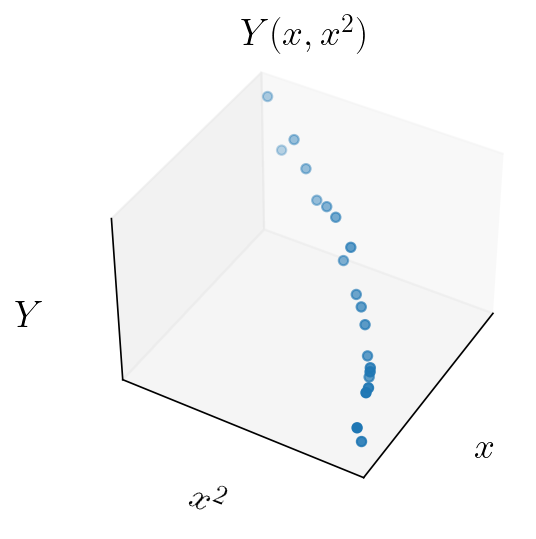
\includegraphics[width=0.3\textwidth]{fnonlin2da}
    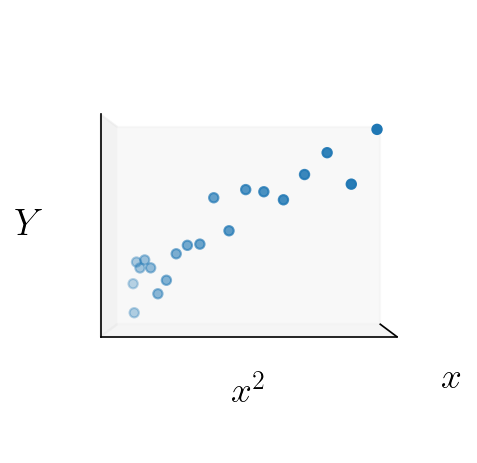
\includegraphics[width=0.3\textwidth]{fnonlin2db}
    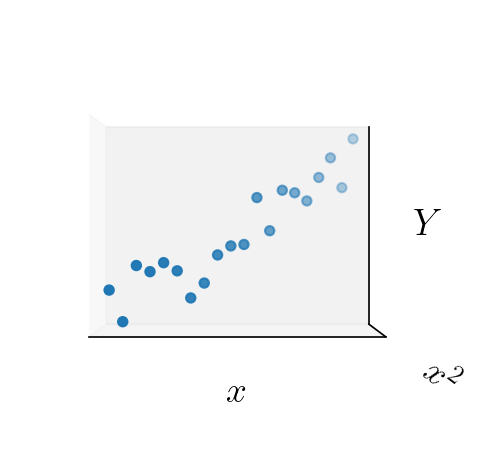
\includegraphics[width=0.3\textwidth]{fnonlin2dc}
  \end{figure}
\note{
  \begin{itemize}
    \item In our case we can map from our scalar feature space to $x' = (x, x^{2})$
    \item We see that relation between $x$ and $y$ stays the same while the $x^{2}$ dimension shows square root characteristics.
  \end{itemize}
}
\end{frame}


\begin{frame}{What if linear is not good enough?}

  \begin{figure}
    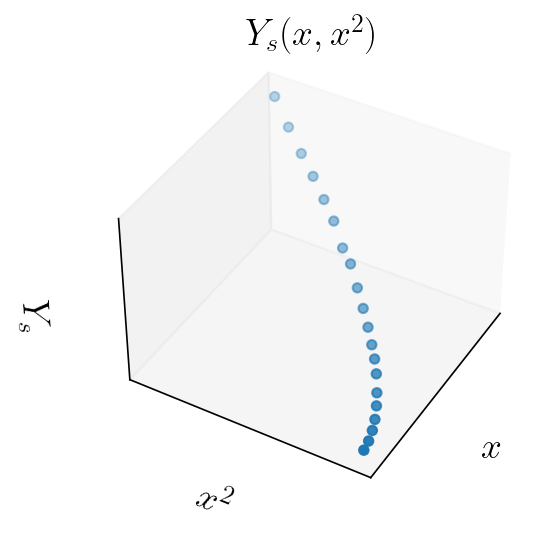
\includegraphics[width=0.3\textwidth]{fsquarenonlin2da}
    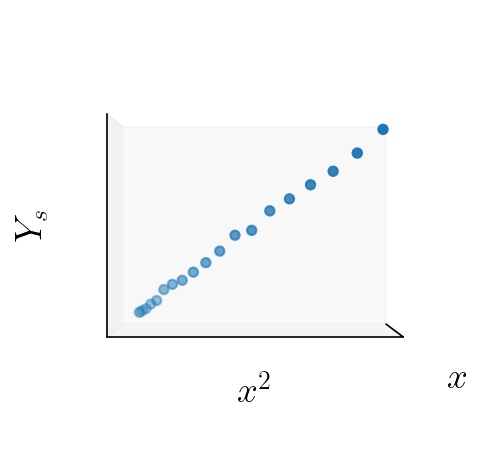
\includegraphics[width=0.3\textwidth]{fsquarenonlin2db}
    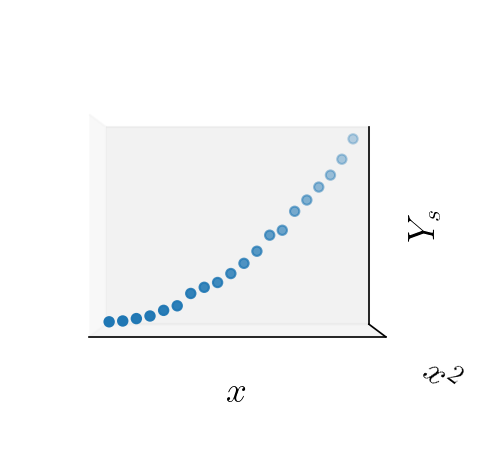
\includegraphics[width=0.3\textwidth]{fsquarenonlin2dc}
  \end{figure}
\note{
  \begin{itemize}
    \item On this slide the underlying $f$ from which the data is generated is $f(x)=x^{2}$.
    \item We see that relation between $x$ and $y$ is polynomial, while the $x^{2}$ dimension now is linear.
  \end{itemize}
}
\end{frame}


\begin{frame}{What if linear is not good enough?}

  \begin{figure}
    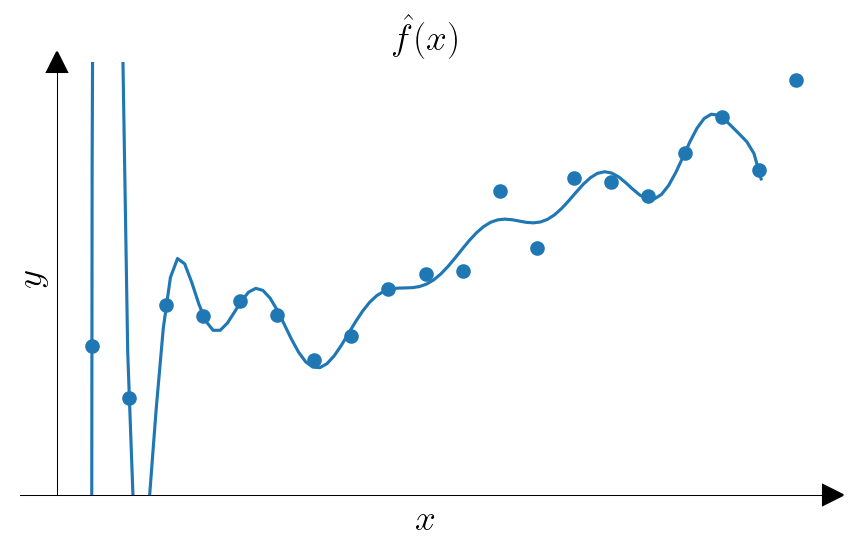
\includegraphics[scale=0.9]{fnonlinfit13}
  \end{figure}

\note{
  \begin{itemize}
    \item This slide shows a 17th degree polynomial fitted to our data from before.
    \item $y=f(x)+\epsilon=\frac{3}{2}x+10+\mathcal{N}(0, 4)$
  \end{itemize}
}
\end{frame}



\begin{frame}{Overfitting}

  \begin{figure}
    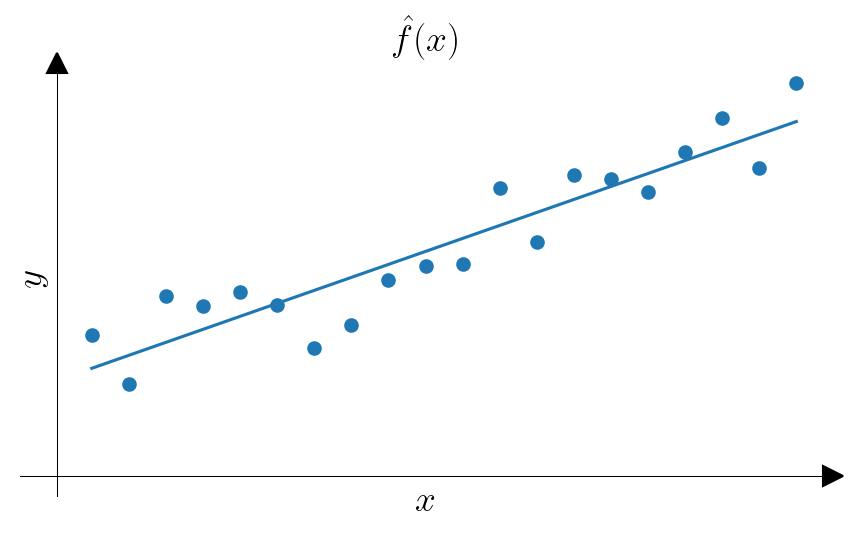
\includegraphics[width=0.4\textwidth]{linregnoticks}
    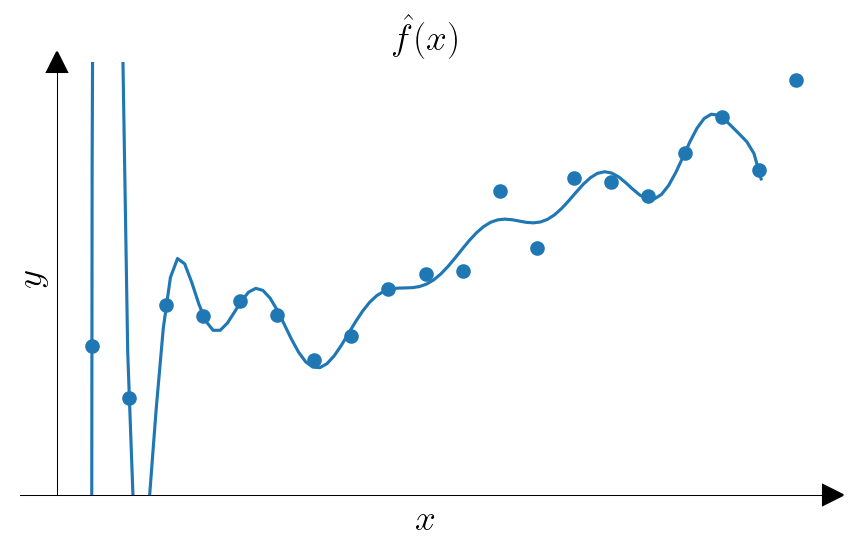
\includegraphics[width=0.4\textwidth]{fnonlinfit13}
  \end{figure}

\note{
  \begin{itemize}
    \item Which of the two estimates of $f$ is better?
    \item $y=f(x)+\epsilon=\frac{3}{2}x+10+\mathcal{N}(0, 4)$
  \end{itemize}
}
\end{frame}


\begin{frame}{Underfitting}

  \begin{figure}
    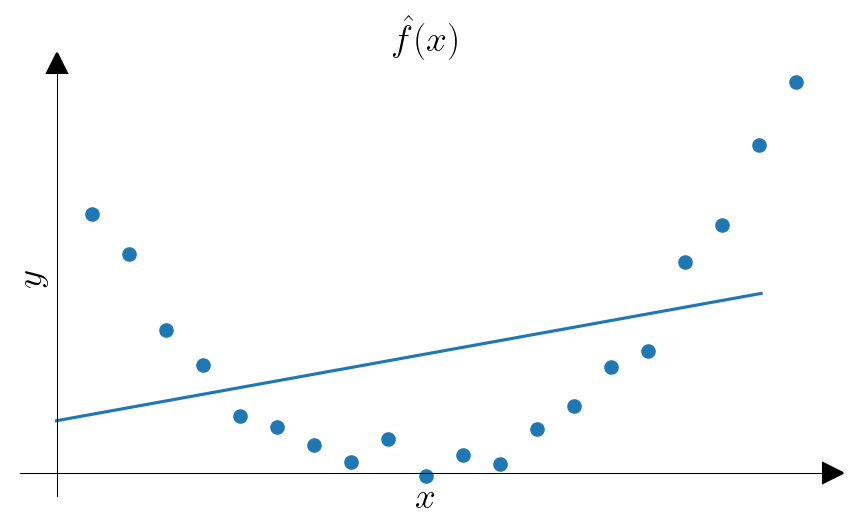
\includegraphics[width=0.4\textwidth]{flnsq}
    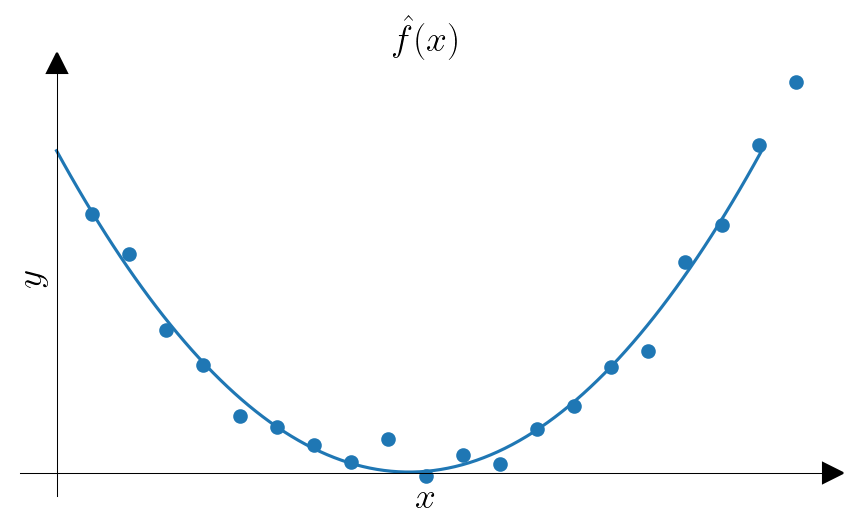
\includegraphics[width=0.4\textwidth]{fsqsq}
  \end{figure}

\note{
  \begin{itemize}
    \item Which of the two estimates of $f$ is better?
    \item $y=f(x)+\epsilon=4(x-10)^{2}+\mathcal{N}(0, 4)$
  \end{itemize}
}
\end{frame}


\begin{frame}{Bias-Variance Trade-Off: Bias}

  \begin{figure}
    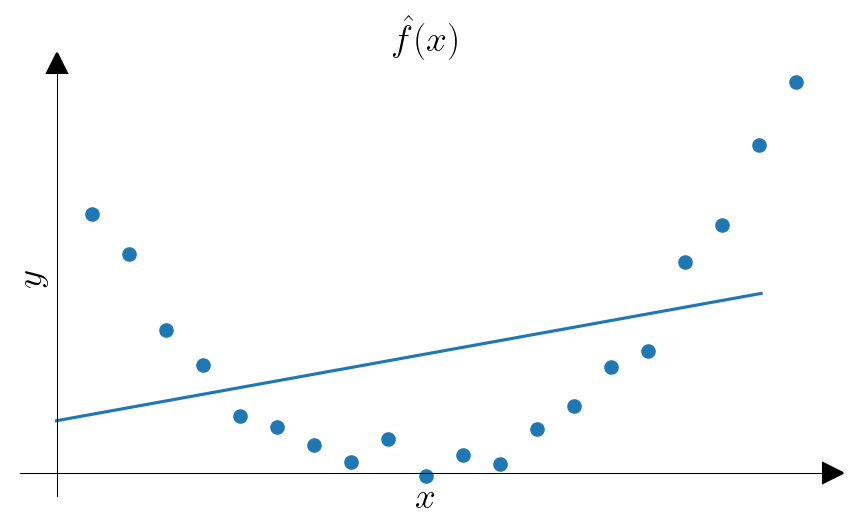
\includegraphics[width=0.4\textwidth]{flnsq}
    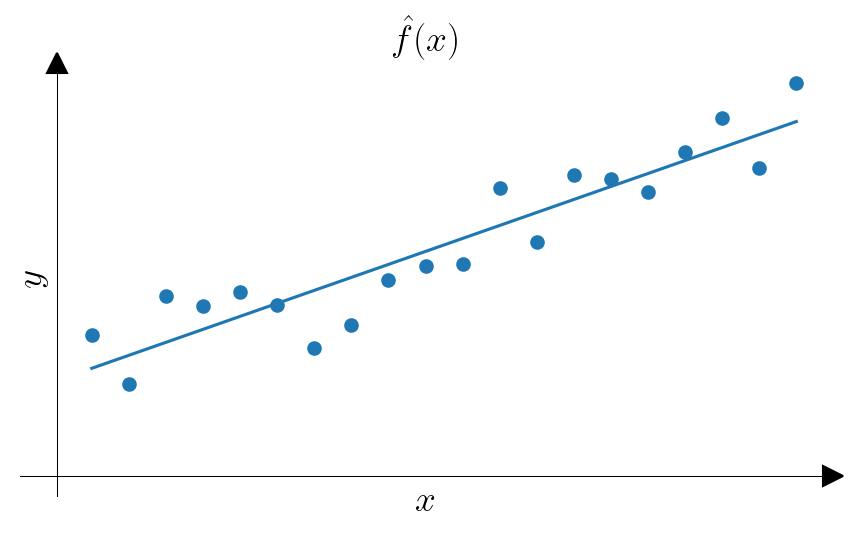
\includegraphics[width=0.4\textwidth]{linregnoticks}
  \end{figure}

\note{
  \begin{itemize}
    \item If we restrict our model e.g. by limiting the complexity we call that bias.
    \item In this case the model is limited to learn linear mappings (high bias).
  \end{itemize}
}
\end{frame}


\begin{frame}{Bias-Variance Trade-Off: Variance}

  \begin{figure}nnnn
    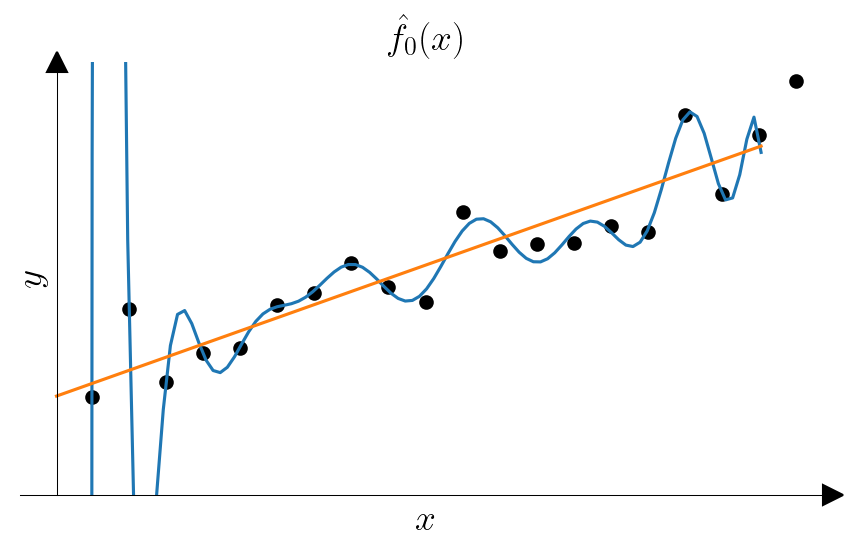
\includegraphics[width=0.3\textwidth]{variance0}
    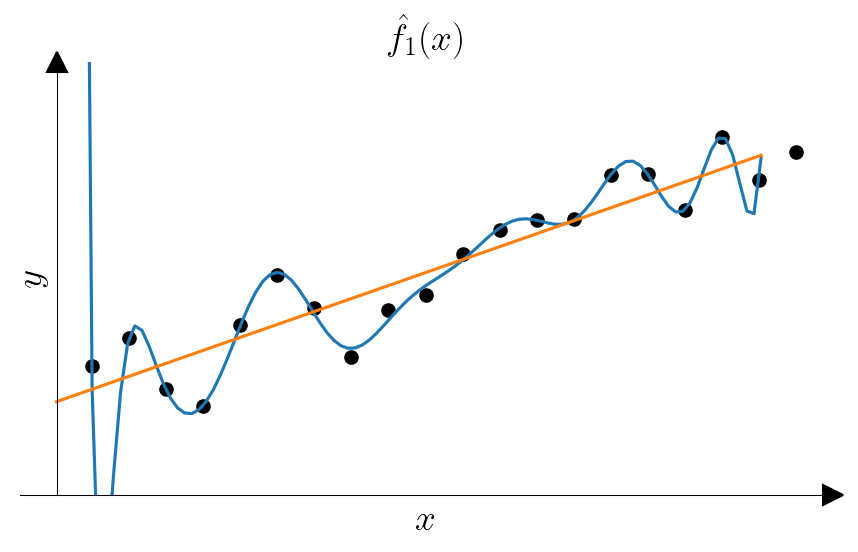
\includegraphics[width=0.3\textwidth]{variance1}
    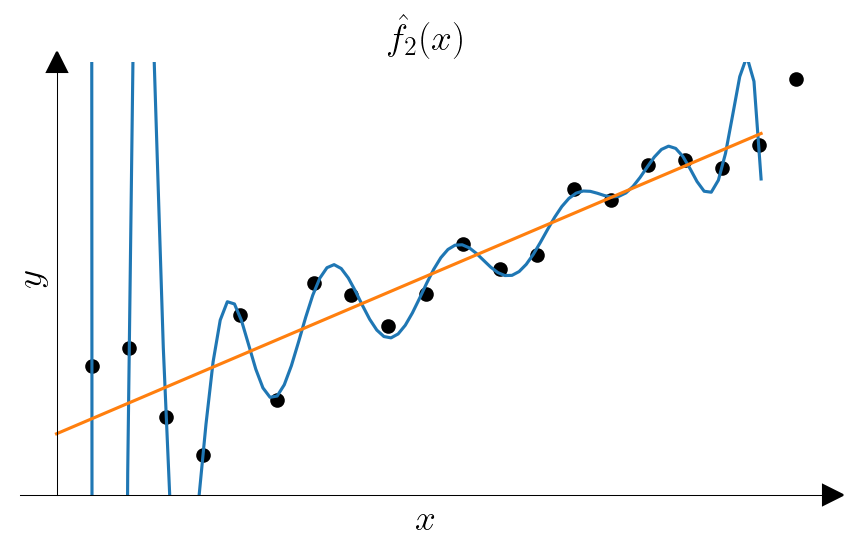
\includegraphics[width=0.3\textwidth]{variance2}
  \end{figure}

\note{
  \begin{itemize}
    \item Three different datasets. Each generated with the linear $f$ we used above.
    \item A 17th degree polynomial is fitted to each of them.
    \item We observe a high variance in the resulting polynomials.
    \item $y=f(x)+\epsilon=\frac{3}{2}x+10+\mathcal{N}(0, 4)$
  \end{itemize}
}
\end{frame}


\begin{frame}{Bias-Variance Trade-Off: Variance}

  \begin{figure}
    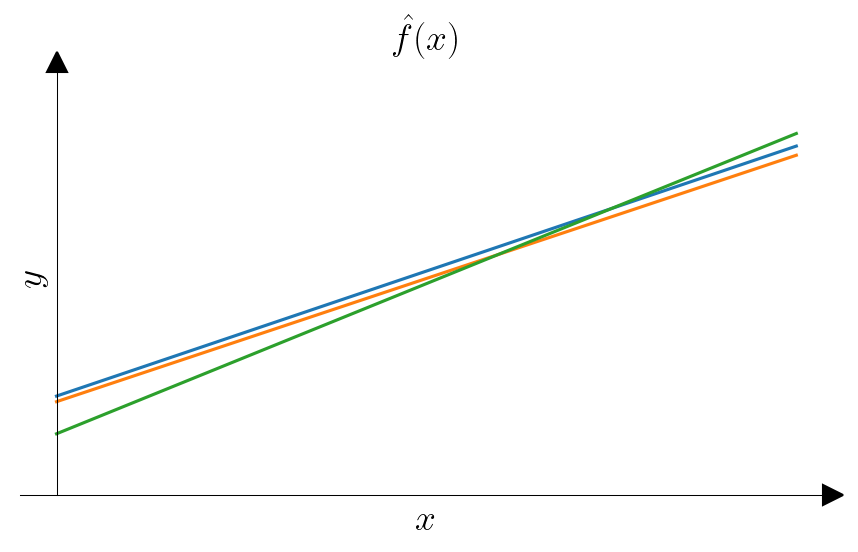
\includegraphics[width=0.4\textwidth]{varianceallln}
    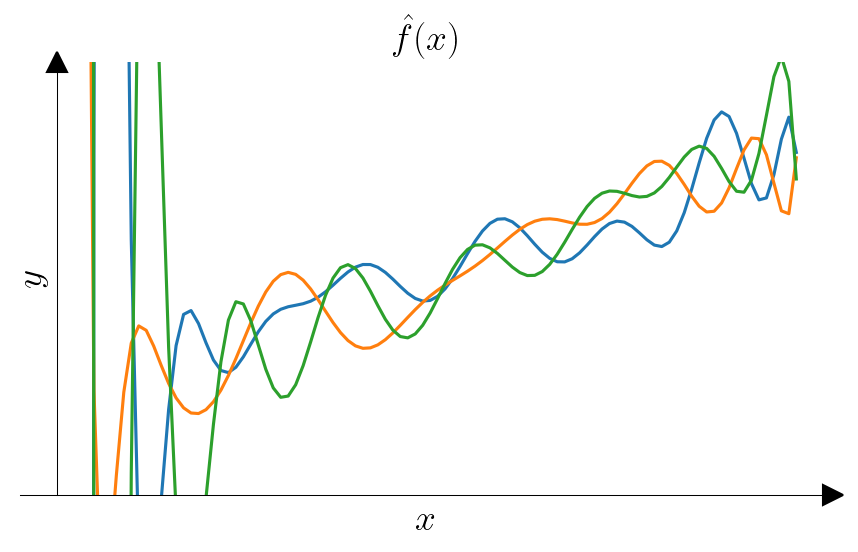
\includegraphics[width=0.4\textwidth]{varianceallsq}
  \end{figure}

\note{
  \begin{itemize}
    \item Three different datasets. Each generated with the linear $f$ we used above.
    \item Comparison on linear models versus polynomial models fitted to the same data.
  \end{itemize}
}
\end{frame}


\begin{frame}{Bias-Variance Trade-Off}

  \begin{figure}
    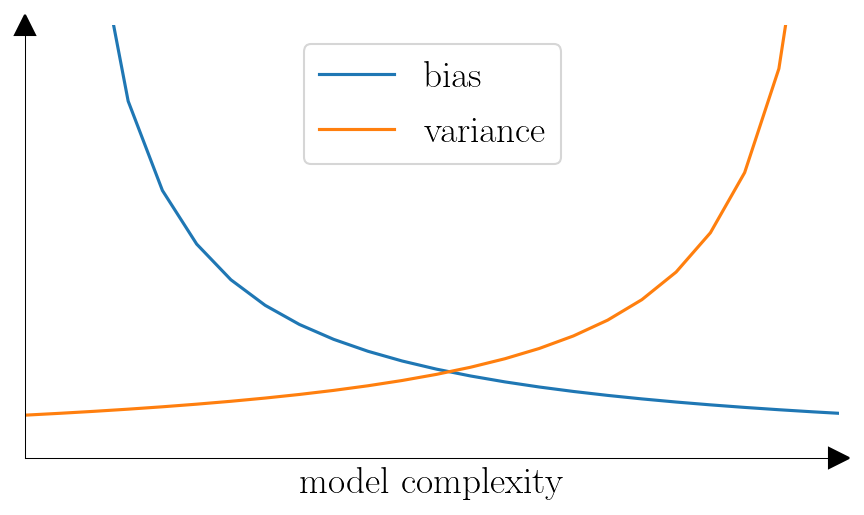
\includegraphics[width=0.9\textwidth]{biasvariance}
  \end{figure}

\note{
  \begin{itemize}
    \item Higher model complexity leads to higher variance and lower bias.
  \end{itemize}
}
\end{frame}


\begin{frame}{Model quality}

  \begin{figure}
    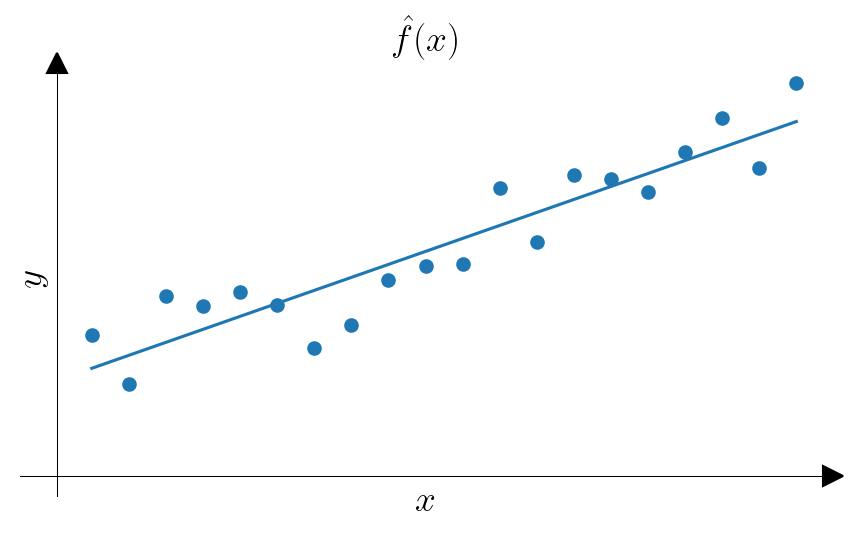
\includegraphics[width=0.4\textwidth]{linregnoticks}
    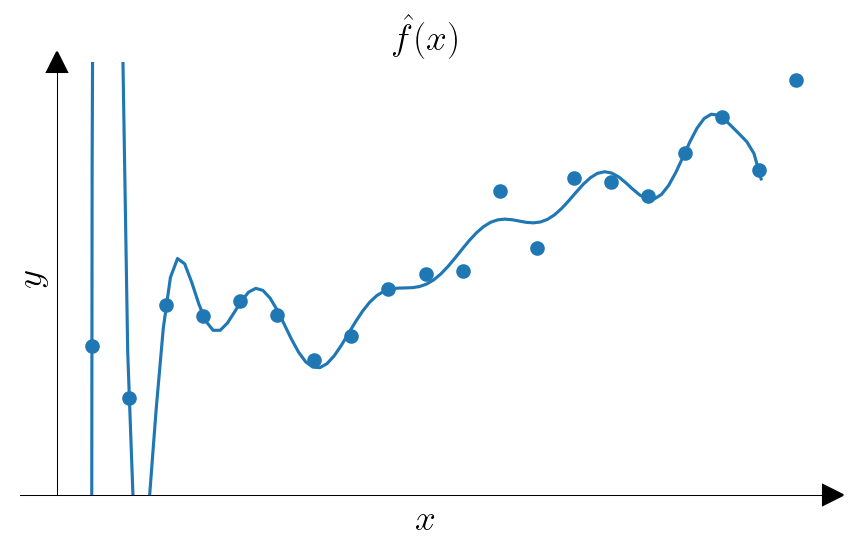
\includegraphics[width=0.4\textwidth]{fnonlinfit13}
  \end{figure}

\note{
  \begin{itemize}
    \item How can we measure the quality of our model?
    \item Which of the two is the better fit?
  \end{itemize}
}
\end{frame}


\begin{frame}{Model quality}
  \begin{equation}
    E = \frac{1}{n}\sum_{i} (y_{i}-\hat{f}(x_{i}))^{2}
  \end{equation}
  \begin{figure}
    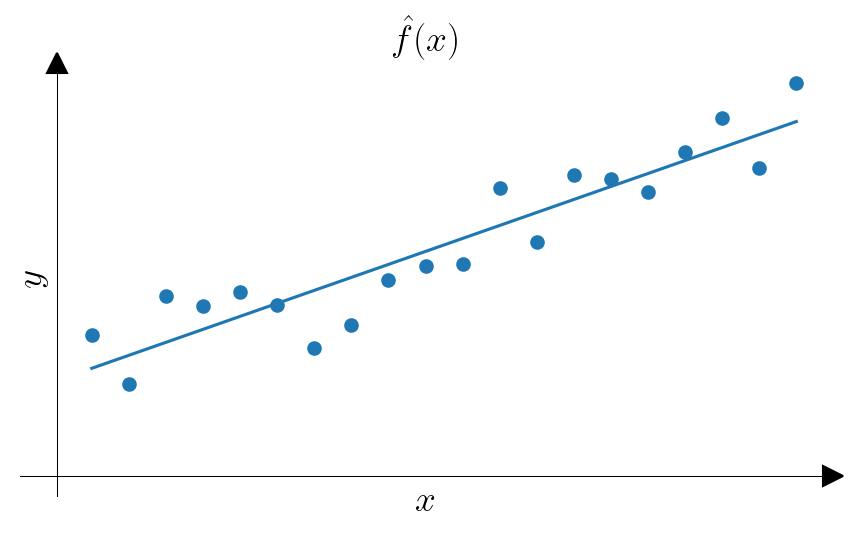
\includegraphics[width=0.4\textwidth]{linregnoticks}
    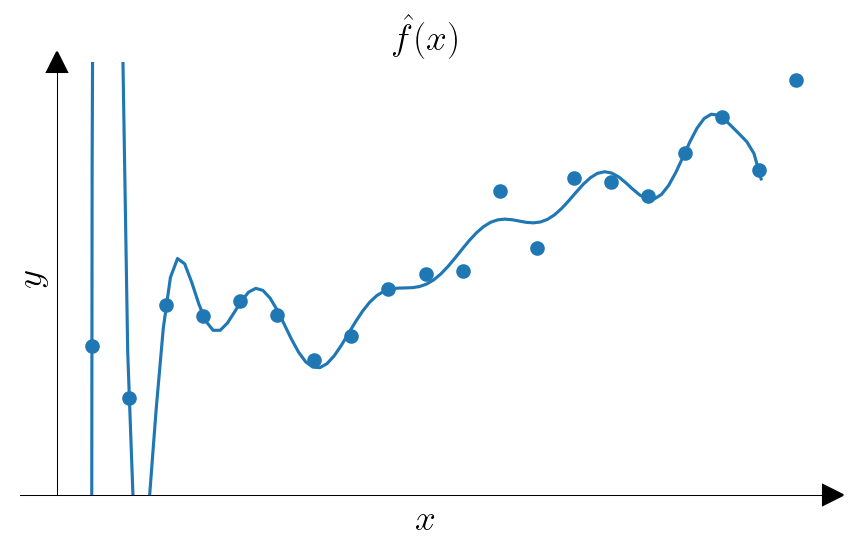
\includegraphics[width=0.4\textwidth]{fnonlinfit13}
  \end{figure}

\note{
  \begin{itemize}
    \item Which of the two has the smaller error (does minimize our objective)? \\
    $rightarrow$ Error becomes smaller with increasing model complexity.
  \end{itemize}
}
\end{frame}


\begin{frame}{Model quality: test dataset}

  \begin{equation}
    E = \frac{1}{n}\sum_{i} (y_{i}-\hat{f}(x_{i}))^{2}
  \end{equation}
  \begin{figure}
    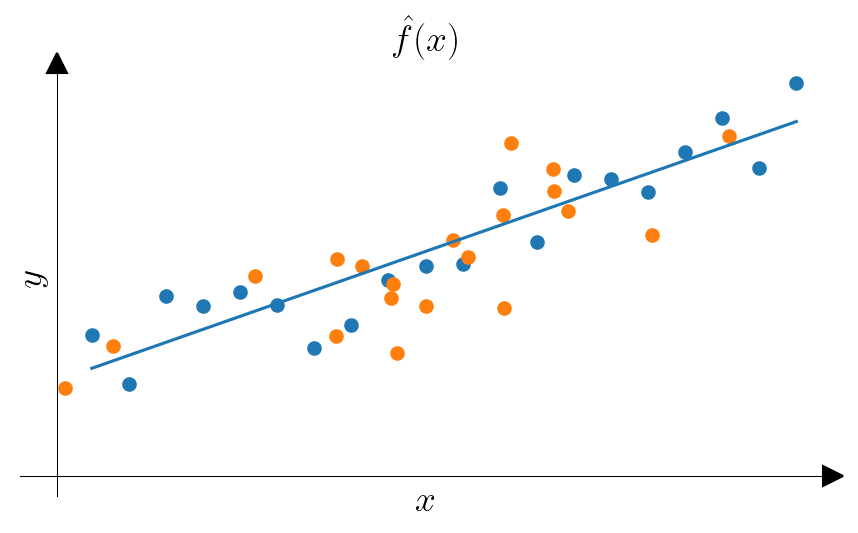
\includegraphics[width=0.4\textwidth]{linval}
    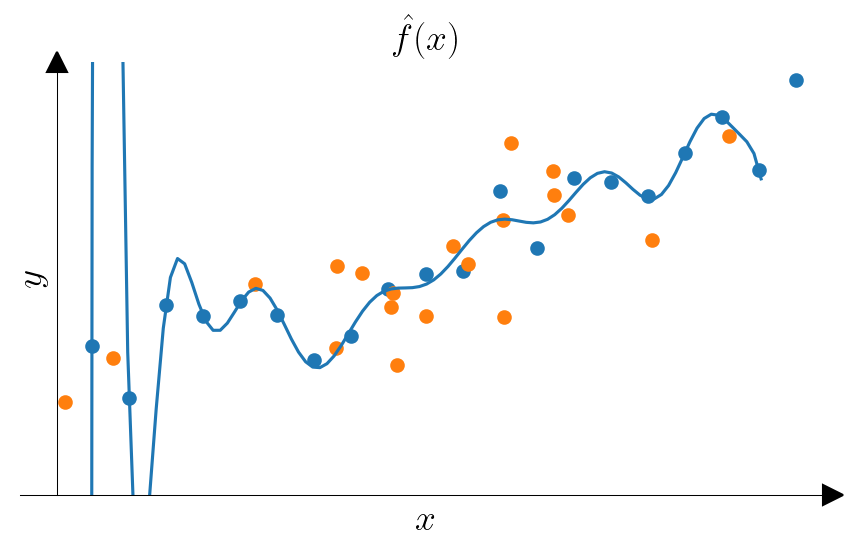
\includegraphics[width=0.4\textwidth]{nonlinval}
  \end{figure}

\note{
  \begin{itemize}
    \item Which of the two has the smaller error (does minimize our objective)?
    \item Split data set before fitting the model and test on unseen data.
    $\rightarrow$  Error shows when model overfits the training data.
  \end{itemize}
}
\end{frame}


\begin{frame}
  \begin{figure}
    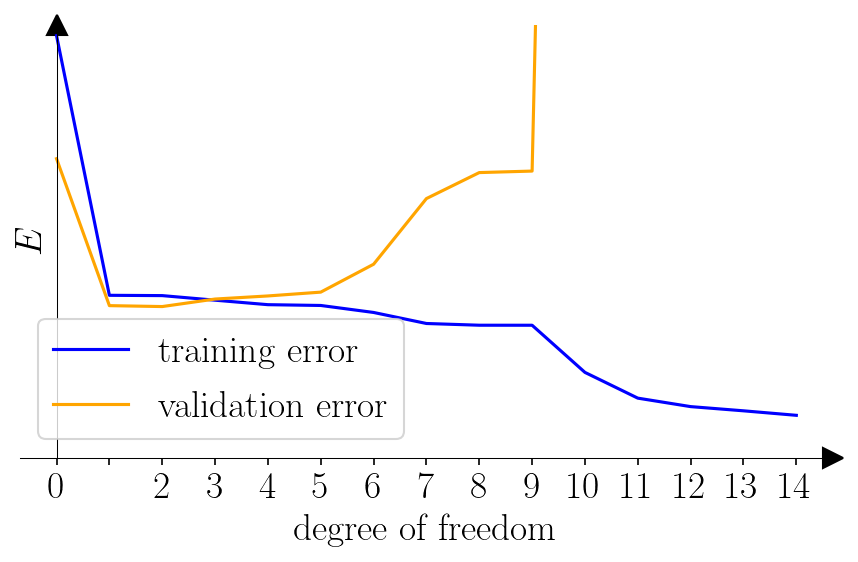
\includegraphics[width=0.9\textwidth]{trainvallin}
  \end{figure}

\note{
  \begin{itemize}
    \item A number of models with increasing complexity was fitted to some training data.
    \item What do you think what form the data generating distribution has?
  \end{itemize}
}
\end{frame}


\begin{frame}
  \begin{figure}
    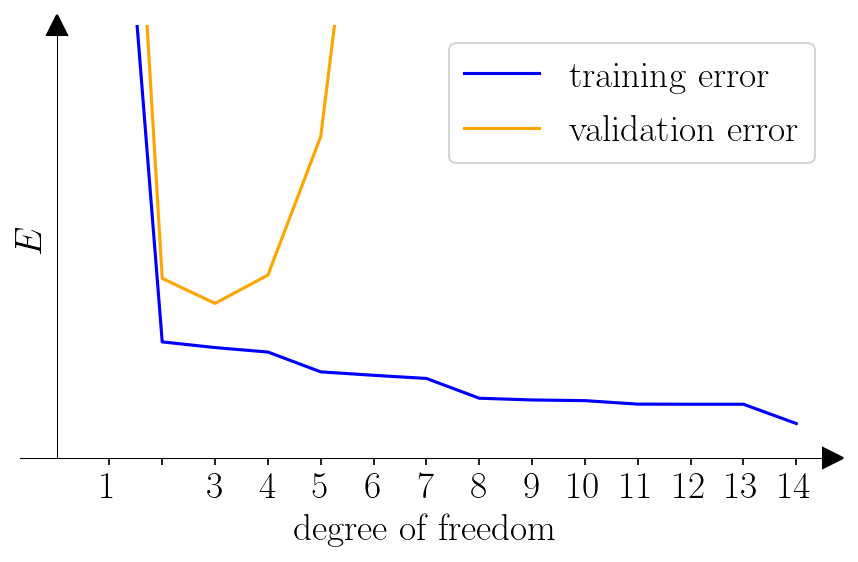
\includegraphics[width=0.9\textwidth]{trainvalpol}
  \end{figure}

\note{
  \begin{itemize}
    \item A number of models with increasing complexity was fitted to some training data.
    \item What do you think what form the data generating distribution has?
  \end{itemize}
}
\end{frame}



\begin{frame}{Classification}

  \begin{figure}
    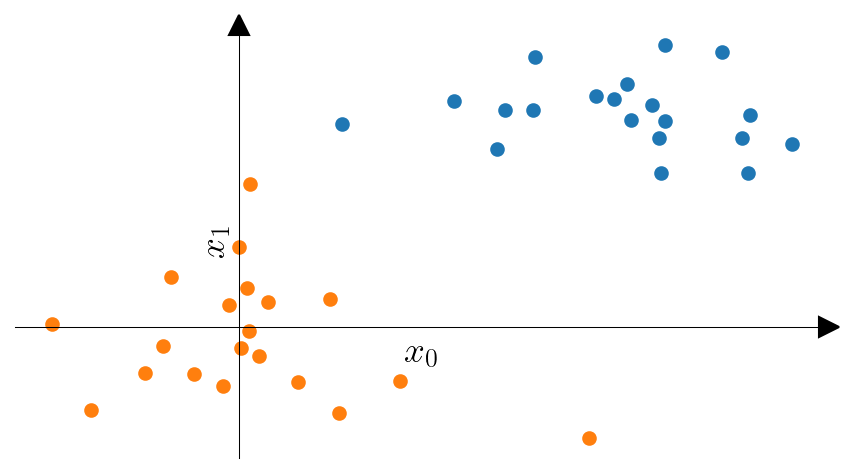
\includegraphics[width=0.9\textwidth]{classification}
  \end{figure}

\note{
  \begin{itemize}
    \item So far we looked at data were the response variable $y$ was quantitative. \\
    $\rightarrow$ This class of problems is referred to as regression problems.
    \item Now we want to look at problems were the response is qualitative or categorical.
    \item Examples: Categorization of facial expressions or objects in images.
  \end{itemize}
}
\end{frame}


\begin{frame}{Classification}
  \begin{figure}
    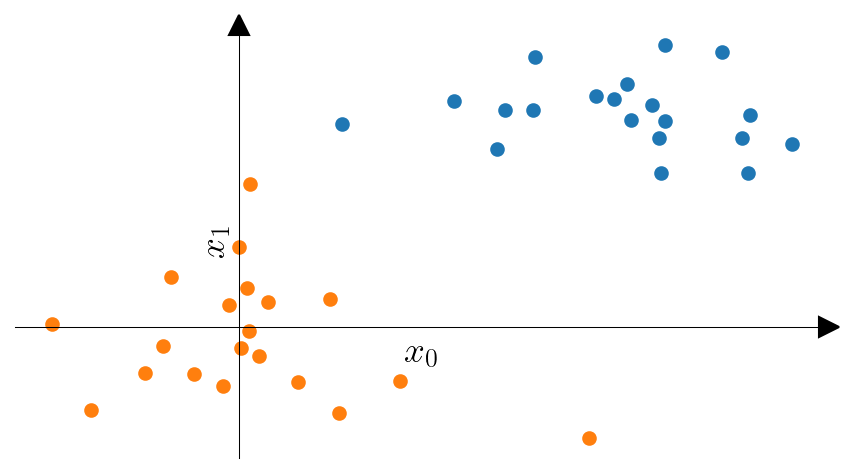
\includegraphics[width=0.9\textwidth]{classification}
  \end{figure}

\note{
  \begin{itemize}
    \item To do this our goal is it to identify a boundary in between a set of training points that separates the two classes.
    \item Whether we call a problem a classification or a regression problem depends only on the response variable.
    \item As for regression, we look only at quantitative predictor variables here.
    \item When the predictor variable is categorical as e.g. in natural language processing they are usually embedded in a quantitative space.
  \end{itemize}
}
\end{frame}


\begin{frame}{Can we solve this with Linear Regression?}

  \begin{figure}
    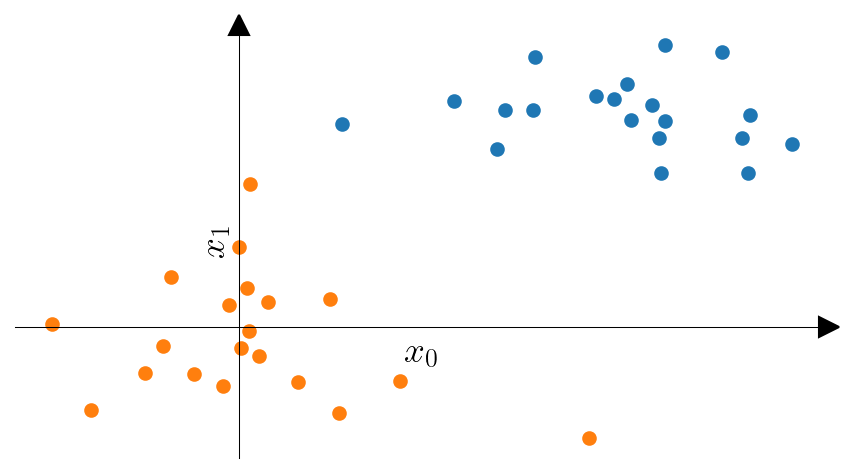
\includegraphics[width=0.9\textwidth]{classification}
  \end{figure}

\note{
  \begin{itemize}
    \item We could define the blue class label as $0$ and the orange class label as $1$ and then apply linear regression.
  \end{itemize}
}
\end{frame}


\begin{frame}{Can we solve this with Linear Regression?}

  \begin{figure}
    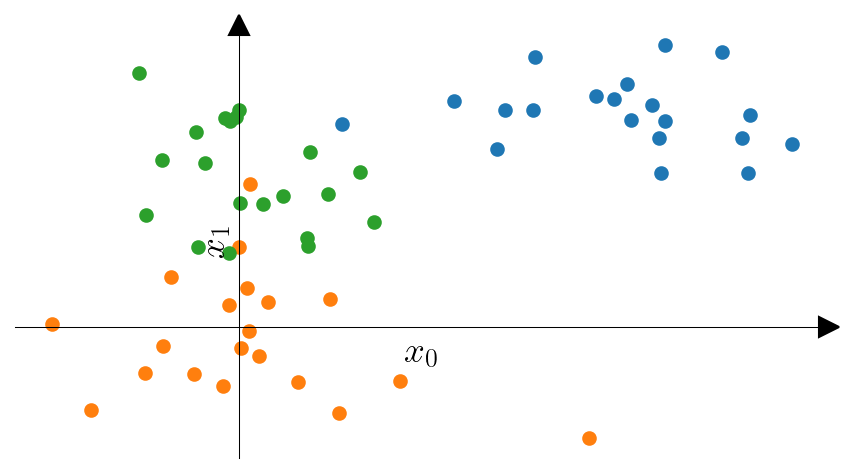
\includegraphics[width=0.9\textwidth]{classification_three}
  \end{figure}

\note{
  \begin{itemize}
    \item However, this would not generalize to more than the binary case.
    \item For three classes we cannot define and order as e.g. orange $>$ blue $>$ green, which would be implied if we would
          assign numbers to our classes as before.
  \end{itemize}
}
\end{frame}


\begin{frame}{Logistic Regression}

  \begin{equation}
    P(class=blue|x)
  \end{equation}
  \begin{figure}
    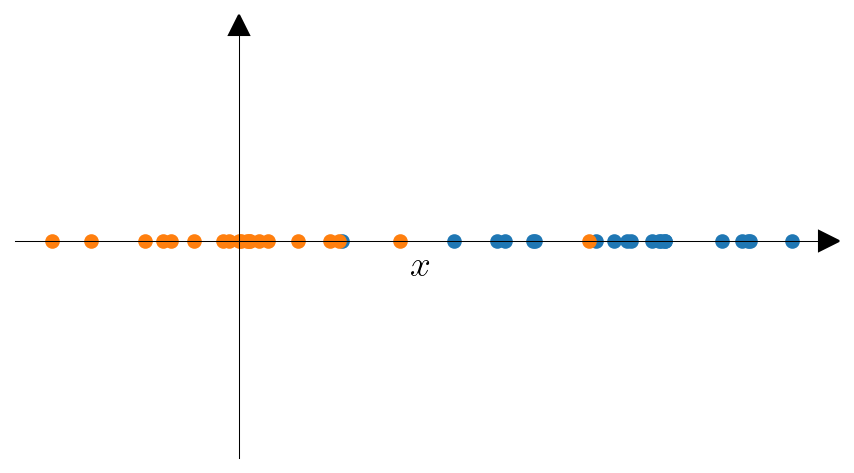
\includegraphics[width=0.9\textwidth]{classification_1d}
  \end{figure}

\note{
  \begin{itemize}
    \item There is a number of algorithms to approach this problem:
          LDA, SVM, Trees, Forests, K-nearest-neighbors, Boosting
    \item For this lecture however, we will first focus on Logistic Regression.
    \item The core idea is to formulate the problem as the regression of a probability function.
    \item This probability connects the predictor variables with the categorical response variable.
    \item For easier illustration, we switch to a two class problem with 1-dimensional input.
  \end{itemize}
}
\end{frame}


\begin{frame}{Logistic Regression}

  % \begin{equation}
  %   p(x) = \alpha x + \beta
  % \end{equation}
  \begin{figure}
    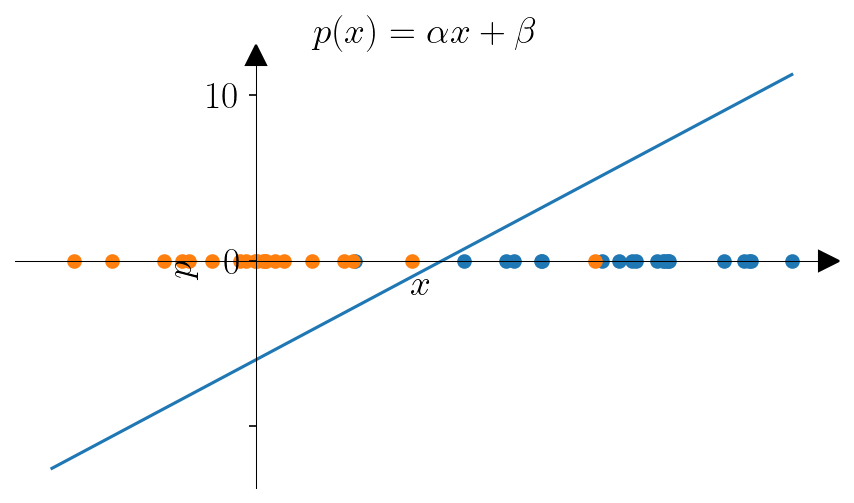
\includegraphics[width=0.8\textwidth]{classification_1d_linp}
  \end{figure}

\note{
  \begin{itemize}
    \item How to model the probability mass function? As a linear mapping as for the regression?
    \item $p$ gets arbitrarily big,  $> 1$ and $< 1$
  \end{itemize}
}
\end{frame}


\begin{frame}{Logistic Regression}

  % \begin{equation}
  %   p(c_{1}|x) = \frac{e^{\alpha x + \beta}}{1+e^{\alpha x + \beta}}
  % \end{equation}
  \begin{figure}
    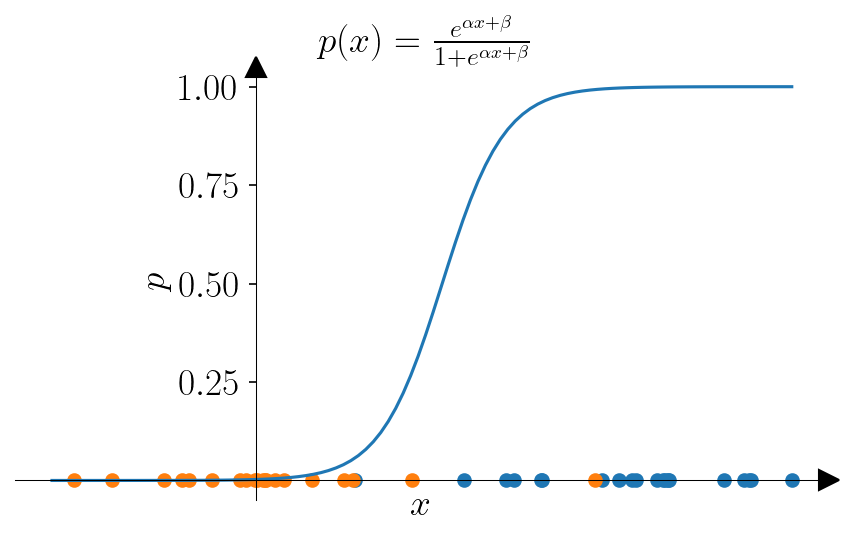
\includegraphics[width=0.8\textwidth]{classification_1d_logp}
  \end{figure}

\note{
  \begin{itemize}
    \item How to model the probability mass function? The logistic function is one of many that makes the result look more like a probability.
  \end{itemize}
}
\end{frame}


\begin{frame}{Logistic Regression}

  \begin{align*}
    p(blue|x) & =\frac{e^{\alpha x + \beta}}{1+e^{\alpha x + \beta}}\\
    p(orange|x) & =1-p(blue|x)
  \end{align*}
  \begin{figure}
    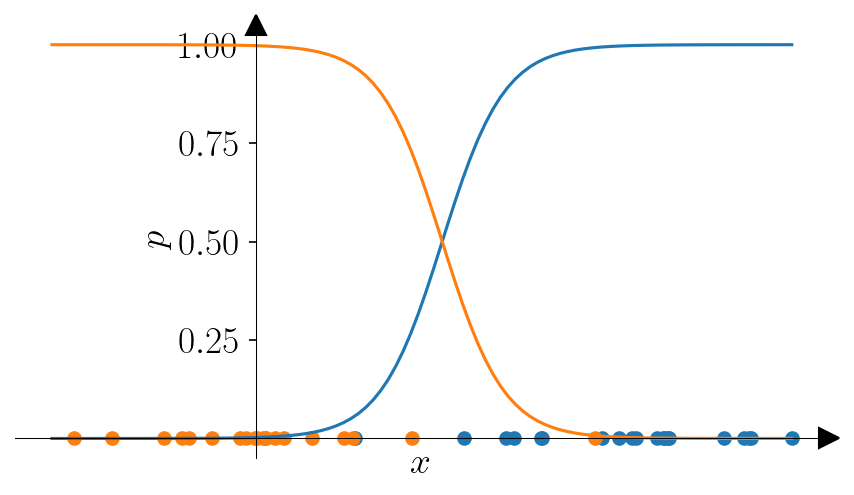
\includegraphics[width=0.7\textwidth]{classification_1d_logp_both}
  \end{figure}

\note{
  \begin{itemize}
    \item How to model the probability mass function? The logistic function is one of many that makes the result look more like a probability.
  \end{itemize}
}
\end{frame}


\begin{frame}{Logistic Regression: Maximum Likelihood}

  % \begin{align*}
  %   y = p(c_{1}|x) = \frac{e^{\alpha x + \beta}}{1+e^{\alpha x + \beta}}
  %   p(c_{0}|x) = 1 - p(c_{1}|x)  = 1 - \frac{e^{\alpha x + \beta}}{1+e^{\alpha x + \beta}}
  % \end{align*}

  \begin{align*}
    p(Y|X,\Theta) &= \prod_{\forall i} p(y_{i}|x_{i}) \\
    \log~p(Y|X,\Theta) &= \sum_{\forall i} \log~p(y_{i}|x_{i}) \\
    E(\Theta) = - \log~p(Y|X,\Theta) &= - \sum_{\forall i} \log~p(y_{i}|x_{i})
  \end{align*}

  % \begin{figure}
  %   \includegraphics[width=0.8\textwidth]{classification_1d_logp}
  % \end{figure}

\note{
  \begin{itemize}
    \item If the samples in our data set are independent and identically distributed (iid assumption) we can write the probability of our dataset beeing generated by our model as a product of the probabilities of the samples.
    \item In our case $\Theta =(\alpha, \beta)$.
    \item If we fix the data and vary the parameters $\Theta$, we call this the likelihood or log-likelihood respectively.
    \item We use the logarithm of the likelihood function for convenience.
    \item We define the error function as the negative log-likelihood and as for the linear regression we can use the derivatives of the error function to determine optimal estimates of $\alpha$ and $\beta$ for the given dataset.
  \end{itemize}
}
\end{frame}


\begin{frame}{Logistic Regression: cross entropy}

  \begin{align*}
    E(\Theta) &= - \sum_{\forall i} q(x) \log~p(y_{i}|x_{i}) = H(q, p)
  \end{align*}

\note{
  \begin{itemize}
    \item The resulting error function describes the cross entropy between the modeled probability distribution and the distribution $q$ which is $1$ if the sample belongs to the respective class and $0$ otherwise.
    \item For further reading we refer to Bishop p48ff.
  \end{itemize}
}
\end{frame}


\begin{frame}{Logistic Regression: softmax}

  \begin{align*}
    p_{i}(x) & = \sigma_{i}(x) = \frac{e^{z_{i}(x)}}{\sum_{\forall j}e^{z_{j}(x)}}
  \end{align*}
with
  \begin{align*}
    z_{i}(x) = \alpha_{i} x + \beta_{i}
  \end{align*}

\note{
  \begin{itemize}
    \item Using the $softmax$ function which is a generalization of the logistic function, we can apply logistic regression to multi class problems.
  \end{itemize}
}
\end{frame}


\begin{frame}{Logistic Regression: softmax}
  \begin{figure}
    \includegraphics[height=5cm]{classification_three_boundaries}
  \end{figure}

g  \begin{equation*}
    p(c|x, \Theta) =
    \begin{pmatrix}
      P(blue|x)\\
      P(orange|x)\\
      P(green|x)
    \end{pmatrix} = \sigma\left (
    \begin{pmatrix}
      \alpha_{00} & \alpha_{01} \\
      \alpha_{10} & \alpha_{11} \\
      \alpha_{20} & \alpha_{21}
    \end{pmatrix} \cdot
    \begin{pmatrix}
      x_0\\
      x_1\\
    \end{pmatrix} +
    \begin{pmatrix}
      \beta_0\\
      \beta_1\\
      \beta_2\\
    \end{pmatrix} \right )
  \end{equation*}

\note{
  \begin{itemize}
    \item Using the $softmax$ function which is a generalization of the logistic function, we can apply logistic regression to multi class problems.
    \item The matrix $\alpha_{ij}$ is often called the weight matrix $W$.
    \item The vector $\beta_{i}$ is often called the bias $b$.
    \item Such a classifier can be and often is written as $y=\sigma(Wx)$ w.l.o.g. using an additional matrix column for the bias.
  \end{itemize}
}
\end{frame}




\begin{frame}{Learning with self-supervision: pretext tasks}

  What objective could that be?

\end{frame}


\begin{frame}{Pretext tasks: Compression}

  \begin{figure}
    \includegraphics[width=0.24\textwidth]{cow_crop}
    \includegraphics[width=0.50\textwidth]{networks_autoencoder}
    \includegraphics[width=0.24\textwidth]{cow_crop}
  \end{figure}

  \note{
    \begin{itemize}
      \item Train an autoencoding network reconstruct an image after coarse feature layer.
      \item Use encoding network for downstream task.
    \end{itemize}
  }

\end{frame}


\begin{frame}{Pretext tasks: Compression + Reconstruction}

  \begin{figure}
    \includegraphics[width=0.24\textwidth]{cow_noise}
    \includegraphics[width=0.50\textwidth]{networks_autoencoder}
    \includegraphics[width=0.24\textwidth]{cow_crop}
  \end{figure}

  \note{
    \begin{itemize}
      \item Same as before but apply distortion function $d(I)$ before feeding the image into the network.
      \item Use encoding network for downstream task.
    \end{itemize}
  }

\end{frame}


\begin{frame}{Pretext tasks: Inpainting}

  \begin{figure}
    \includegraphics[width=0.24\textwidth]{cow_inpainting_00}
    \includegraphics[width=0.50\textwidth]{networks_autoencoder}
    \includegraphics[width=0.24\textwidth]{cow_inpainting_01}
  \end{figure}

  \note{
    \begin{itemize}
      \item Predict one part of the data from another.
      \item Can also be a random part of the image or e.g. the bottom half or frames of a video sequence.
      \item Context Encoders: Feature Learning by Inpainting, Pathak et al., CVPR 2016
    \end{itemize}
  }

\end{frame}


\begin{frame}{Pretext tasks: Colorization}

  \begin{figure}
    \includegraphics[width=0.24\textwidth]{cow_crop_grey}
    \includegraphics[width=0.50\textwidth]{networks_autoencoder}
    \includegraphics[width=0.24\textwidth]{cow_crop}
  \end{figure}

  \note{
    \begin{itemize}
      \item Similar to inpainting we predict a left-out property the data.
      \item Colorful Image Colorization, Zhang et al., ECCV 2016
      \item Tracking Emerges by Colorizing Videos, Vondrick et al., ECCV 2018
    \end{itemize}
  }

\end{frame}


\begin{frame}{Pretext tasks: Frame permutation}

  \begin{columns}
    \begin{column}{0.33\textwidth}
      \begin{figure}
        \includegraphics[width=0.45\textwidth]{cow_crop-0-1}\hspace{0.2mm}\includegraphics[width=0.45\textwidth]{cow_crop-1-0}\\%
        \includegraphics[width=0.45\textwidth]{cow_crop-1-1}\hspace{0.2mm}\includegraphics[width=0.45\textwidth]{cow_crop-0-0}
      \end{figure}
    \end{column}
    \begin{column}{0.43\textwidth}
      \begin{figure}
        \includegraphics[width=0.99\textwidth]{networks_encoder}
      \end{figure}
    \end{column}
    \begin{column}{0.23\textwidth}
      \begin{align*}
        {4, 2, 1, 3}
      \end{align*}
    \end{column}
  \end{columns}

  \note{
    \begin{itemize}
      \item We can also formulate the pretext task as classification problem. Here one of $n!$ possible permutations.
      \item Can also be done with video frames.
      \item Unsupervised Learning of Visual Representations by Solving Jigsaw Puzzles, Noroozi \& Favaro, ECCV 2016
    \end{itemize}
  }


\end{frame}


\begin{frame}{Pretext tasks: Frame relation}

    \begin{columns}
    \begin{column}{0.33\textwidth}
      \begin{figure}
        \includegraphics[width=0.45\textwidth]{cow_crop-0-1}\hspace{0.2mm}\includegraphics[width=0.45\textwidth]{cow_crop-1-0}\\%
      \end{figure}
    \end{column}
    \begin{column}{0.43\textwidth}
      \begin{figure}
        \includegraphics[width=0.99\textwidth]{networks_encoder}
      \end{figure}
    \end{column}
    \begin{column}{0.23\textwidth}
      \begin{align*}
        top-right
      \end{align*}
    \end{column}
  \end{columns}

  \note{
    \begin{itemize}
      \item Or as a discrete spatial relation
      \item Unsupervised Visual Representation Learning by Context Prediction, Doersch et al., ICCV 2015
    \end{itemize}
  }

\end{frame}


\begin{frame}{Pretext tasks: Transfer knowledge}

  \begin{figure}
    \includegraphics[height=0.9\textheight]{tl_00}
  \end{figure}

  \note{
    \begin{itemize}
      \item Same as for transfer learning with supervised pretraining.
      \item Replace some layers, fine tune some layers.
    \end{itemize}
  }

\end{frame}


\begin{frame}{Pretext tasks: Transfer knowledge}
  \begin{figure}
    \includegraphics[width=0.85\textwidth]{pretext_performance}
  \end{figure}
  \note{
    \begin{itemize}
      \item Problem: learned representations are very task specific
    \end{itemize}
  }
\end{frame}

\begin{frame}{Energy-based self-supervised representation learning}

  \begin{align*}
    similarity(x_{i}, x_{j}) > similarity(x_{i}, x_{k}) \Rightarrow energy(e_{i}, e_{j}) < energy(e_{i}, e_{k})
  \end{align*}

  \begin{figure}
    \includegraphics[width=0.4\textwidth]{energy_siamese}
  \end{figure}

  \note{
    \begin{itemize}
      \item For energy-based learning we often use what is called Siamese networks.
      \item Two (almost) identical networks, that share weights.
      \item We could summarize the methods in this chapter also as Siamese Representation Learning.
      \item If the inputs to the two networks are compatible in some way, the energy should be low, otherwise high.
      \item Similarity does not mean similar appearance in pixel space.
    \end{itemize}
  }

\end{frame}


\begin{frame}{Contrastive Learning}

  \begin{figure}
    \includegraphics[width=0.9\textwidth]{pirl}
  \end{figure}

  \note{
    \begin{itemize}
      \item Image from Self-Supervised Learning of Pretext-Invariant Representations, Misra \& Maaten, CVPR 2020
    \end{itemize}
  }

\end{frame}


\begin{frame}{Contrastive Learning}

  \begin{figure}
    \includegraphics[width=0.9\textwidth]{pirl_layers}
  \end{figure}

  \note{
    \begin{itemize}
      \item Image from Self-Supervised Learning of Pretext-Invariant Representations, Misra \& Maaten, CVPR 2020
    \end{itemize}
  }

\end{frame}


\begin{frame}{Contrastive Learning}

  \begin{figure}
    \includegraphics[width=0.9\textwidth]{simclr_distortions}
  \end{figure}

  \note{
    \begin{itemize}
      \item Image from A Simple Framework for Contrastive Learning of Visual Representation, Chen et al., ICML 2020
    \end{itemize}
  }

\end{frame}


\begin{frame}{Contrastive Learning}

  Good negative samples are very important
  \begin{itemize}
    \item Have huge batch sizes
    \item Use memory banks (momentum of activations)
    \item Momentum on the weights of the siamese twin
  \end{itemize}


  \note{
    \begin{itemize}
      \item Huge batch sizes are easy to implement but have heavy compute demands  \\
            A Simple Framework for Contrastive Learning of Visual Representations, Chen et al., ICML 2020
      \item Compute efficient but memory bank needs a lot of RAM \\
            Unsupervised Feature Learning via Non-Parametric Instance-level Discrimination, Wu et al., CVPR 2018
      \item Saves memory but needs extra forward pass \\
            Momentum Contrast for Unsupervised Visual Representation Learning, He et al., CVPR 2020
    \end{itemize}
  }

\end{frame}


\begin{frame}{Non-Contrastive Learning}

  There are other ways to approach this (clustering, distillation)
  \begin{itemize}
    \item DeepCluster, Sela, SwAV
    \item BYOL, SimSiam
  \end{itemize}

  \note{
    \begin{itemize}
      \item We are gonna skip those for today. Unfortunately we can't talk about everything :(
      \item There is a very nice lecture by Ishan Misra though, if you want to learn more: \url{https://www.youtube.com/watch?v=8L10w1KoOU8}
    \end{itemize}
  }

\end{frame}


\begin{frame}{Redundancy Reduction Learning}

  \begin{align*}
    f_{i}(I) &= f_{i}(d(I))\\
    f_{i}(I) &\neq f_{j}(d(I))
  \end{align*}

  \note{
    \begin{itemize}
      \item This equations are a dramatically oversimplified sketch of the idea.
      \item While neurons should respond the same to an image and its distorted version, they should all respond differently.
      \item We don't have spare neurons, so we don't want redundancy in their activations.
      \item Possible principles underlying the transformation of sensory messages, Horace Barlow, 1961
    \end{itemize}
  }

\end{frame}


\begin{frame}{Barlow Twins}

  \begin{figure}
    \includegraphics[width=0.9\textwidth]{barlow_twins}
  \end{figure}

  \note{
    \begin{itemize}
      \item Our objective is to make the correlation matrix a diagonal matrix.
      \item To prevent constant but decorrelated output, $Z_{a}$ and $Z_{b}$ are standardized before the correlation matrix is computed.
      \item Image from Barlow Twins: Self-Supervised Learning via Redundancy Reduction, Zbontar et al., ICML 2021
    \end{itemize}
  }

\end{frame}


\begin{frame}{Barlow Twins}

  \begin{figure}
    \includegraphics[height=0.9\textheight]{barlow_twins_algo}
  \end{figure}

  \note{
    \begin{itemize}
      \item Image from Barlow Twins: Self-Supervised Learning via Redundancy Reduction, Zbontar et al., ICML 2021
    \end{itemize}
  }

\end{frame}



% \begin{frame}{SEER}

%   \note{
%     \begin{itemize}
%       \item
%     \end{itemize}
%   }

% \end{frame}

\begin{frame}{Generative Learning}

  What's generative learning?

\end{frame}

\begin{frame}{Generative Learning}

  We want to model the data distribution $p(x)$ directly.

  \note{
    \begin{itemize}
      \item Where $x$ is a sample image.
      \item How is this even possible? Let's see ...
    \end{itemize}
  }

\end{frame}


\begin{frame}{PixelRNN/PixelCNN}

  \begin{align*}
    p(x) = p(x_{1}, ..., x_{n}) = \prod_{i}^{n^{2}} p(x_{i})p(x_{i}|x_{1}, ..., x_{i-1})
  \end{align*}

  \begin{figure}
    \includegraphics[width=0.3\textwidth]{pixelrnn_pixels}
  \end{figure}

  \note{
    \begin{itemize}
      \item Fully Visible Belief Network
      \item Product of distributions using chain rule (decompose likelihood of an image into pixel probabilities).
      \item Train RNN to classify pixels (e.g. 1 out of 255).
      \item Also possible to formulate as CNN, but still one forward pass per pixel necessary at test time.
      \item Image from Pixel Recurrent Neural Networks, van den Oord, ICML 2016
    \end{itemize}
  }
\end{frame}


\begin{frame}{Modeling using a latent variable}

  \begin{columns}
    \hspace{2cm}
    \begin{column}{0.3\textwidth}
      \begin{align*}
        z = \begin{pmatrix}
          haircolor \\
          skin tone \\
          beard \\
          gender \\
          classes \\
          expression
        \end{pmatrix}
      \end{align*}
    \end{column}
    \begin{column}{0.1\textwidth}
      \begin{align*}
        \Rightarrow
      \end{align*}
    \end{column}
    \begin{column}{0.4\textwidth}
      \begin{figure}
        \includegraphics[width=.6\textwidth]{vae_faces}
      \end{figure}
    \end{column}
    \hspace{2cm}
  \end{columns}

  \note{
    \begin{itemize}
      \item Image from Auto-Encoding Variational Bayes, Kingma \& Welling, ICLR 2014
      \item
    \end{itemize}
  }

\end{frame}


\begin{frame}{Modeling using a latent variable}

  \begin{align*}
    p_{\theta}(x) = \int p_{\theta}(x|z)p_{\theta}(z) dz
  \end{align*}

  \begin{columns}
    \hspace{2cm}
    \begin{column}{0.3\textwidth}
      \begin{align*}
        z = \begin{pmatrix}
          haircolor \\
          skin tone \\
          beard \\
          gender \\
          classes \\
          expression
        \end{pmatrix}
      \end{align*}
    \end{column}
    \begin{column}{0.1\textwidth}
      \begin{align*}
        \Rightarrow
      \end{align*}
    \end{column}
    \begin{column}{0.4\textwidth}
      \begin{figure}
        \includegraphics[width=.6\textwidth]{vae_faces}
      \end{figure}
    \end{column}
    \hspace{2cm}
  \end{columns}

  \note{
    \begin{itemize}
      \item $p_{\theta}$ is the data likelihood we want to maximize.
      \item We can approximate $p(z)$ e.g. as Gaussian.
      \item We can learn $p(x|z)$ e.g. with a generator network.
      \item However, the integral over $z$ is intractable.
    \end{itemize}
  }

\end{frame}


\begin{frame}{ELBO (evidence lower bound)}

  \begin{align*}
    E_{q(z|x)} \log p(x|z) - KL(q(z|x)||p(z))
  \end{align*}

  \note{
    \begin{itemize}
      \item Luckily it turns out that this term is a lower bound on our intractable data likelihood.
      \item $KL$ is the Kullback-Leibler divergence, a similarity measurement for probability distributions.
      \item $q(z|x)$ is a tractable approximation of the intractable $p(z|x)$.
      \item Yes, there is a lot of math we just skipped. You can find a full derivation here: \url{https://www.youtube.com/watch?v=uaaqyVS9-rM&t=1182s}
    \end{itemize}
  }

\end{frame}


\begin{frame}{ELBO (evidence lower bound)}

  \begin{align*}
    E_{q(z|x)} \log p(x|z) - KL(q(z|x)||p(z))
  \end{align*}

  \vspace{2cm}

  \center{\huge{Let's maximize it!}}

  \note{
    \begin{itemize}
      \item Luckily it turns out that this term is a lower bound on our intractable data likelihood.
      \item $KL$ is the Kullback-Leibler divergence, a similarity measurement for probability distributions.
      \item $q(z|x)$ is a tractable approximation of the intractable $p(z|x)$.
    \end{itemize}
  }

\end{frame}


\begin{frame}{Variational Autoencoder (VAE)}

  \begin{align*}
    q(z|x) = \mathcal{N}(\mu_{z}, \sigma_{z})
  \end{align*}

  \begin{figure}
    \includegraphics[width=0.9\textwidth]{networks_vae_recognition}
  \end{figure}

  \note{
    \begin{itemize}
      \item Let's just assume the $p(z)$ is gaussian distributed.
      \item And let's additionally assume all elements of $z$ are independent.
      \item To approximate $q(z|x)$ we learn a mapping with a neural net.
      \item This is the encoder part of the variational autoencoder (sometimes called recognition model).
    \end{itemize}
  }

\end{frame}


\begin{frame}{Variational Autoencoder (VAE)}

  \begin{align*}
    MSE(x,\hat{x})
  \end{align*}

  \begin{figure}
    \includegraphics[width=0.9\textwidth]{networks_vae_generator}
  \end{figure}

  \note{
    \begin{itemize}
      \item minimize $MSE(x,\hat{x})$ to maximize $E_{q(z|x)} \log p(x|z)$
      \item This is the decoder part of the variational autoencoder (sometimes called generator model).
    \end{itemize}
  }

\end{frame}


\begin{frame}{Variational Autoencoder (VAE)}

  \begin{figure}
    \includegraphics[width=0.9\textwidth]{networks_vae_full}
  \end{figure}

  \note{
    \begin{itemize}
      \item Full VAE architecture for training.
    \end{itemize}
  }

\end{frame}


\begin{frame}{VAE: Reparameterization Trick}

  \begin{align*}
    z = \mu_{z}+\epsilon\sigma_{z}~with~\epsilon ~ \mathcal{N}(0, 1)
  \end{align*}

  \begin{figure}
    \includegraphics[width=0.9\textwidth]{networks_vae_full}
  \end{figure}

  \note{
    \begin{itemize}
      \item We cannot backpropagate through $z \sim \mathcal{N}(\mu_{z}, \sigma_{z})$
      \item Therefor we set to $z=\mu_{z}+\epsilon\sigma_{z}$ with $\epsilon ~ \mathcal{N}(0, 1)$
      \item This is called the reparameterization trick.
    \end{itemize}
  }

\end{frame}


\begin{frame}{Variational Autoencoder (VAE)}

  \begin{figure}
    \includegraphics[width=0.9\textwidth]{vae_zviz}
  \end{figure}

  \note{
    \begin{itemize}
      \item At test time we draw $z$ from $p(z)=\mathcal{N}(0, 1)$.
      \item Enforcing $KL(q(z|x)||p(z))$ leads to a smooth latent state.
      \item Image from \url{https://towardsdatascience.com/intuitively-understanding-variational-autoencoders-1bfe67eb5daf}
    \end{itemize}
  }

\end{frame}


\begin{frame}{Variational Autoencoder (VAE)}

  \begin{figure}
    \includegraphics[width=0.5\textwidth]{vae_mnist}
  \end{figure}

  \note{
    \begin{itemize}
      \item A VAE trained to generate MNIST digits.
      \item A grid in the latent space leads to consistent generations in pixelspace.
      \item Image from Auto-Encoding Variational Bayes, Kingma \& Welling, ICLR 2014
    \end{itemize}
  }

\end{frame}



\begin{frame}{Adversarial Learning}

  \begin{columns}
    \begin{column}{0.25\textwidth}
      \begin{figure}
        \includegraphics[width=0.9\textwidth]{cow_grey}
      \end{figure}
    \end{column}
    \begin{column}{0.45\textwidth}
      \begin{figure}
        \includegraphics[width=1.0\textwidth]{networks_autoencoder}
      \end{figure}
    \end{column}
    \begin{column}{0.25\textwidth}
      \begin{figure}
        \includegraphics[width=0.9\textwidth]{cow_orig}
      \end{figure}
    \end{column}
  \end{columns}

  \note{
    \begin{itemize}
      \item If we have a generated image (e.g. from the VAE or from colorizing a grey scale image), we do not actually care if the image is exactly the same as the input image.
      \item We just want it to be realistic. But the MSE forces the output to be the same as the reference.
    \end{itemize}
  }
\end{frame}


\begin{frame}{Adversarial Learning}

  \begin{columns}
    \begin{column}{0.95\textwidth}
      \begin{figure}
        \includegraphics[width=.99\textwidth]{networks_adversarial_loss}
      \end{figure}
    \end{column}
    \begin{column}{0.05\textwidth}
      \begin{align*}
        Fake/Real
      \end{align*}
    \end{column}
  \end{columns}

  \note{
    \begin{itemize}
      \item Instead of formulating a good error measurement ourselves, we can train a classifier to distinguish between a real image and a generated (fake) image.
      \item This way we do not measure if the image looks similar to the original but only if the image looks realistic.
    \end{itemize}
  }
\end{frame}


\begin{frame}{Adversarial Learning}

  \begin{columns}
    \begin{column}{0.95\textwidth}
      \begin{figure}
        \includegraphics[width=.99\textwidth]{networks_adversarial_loss_gradient}
      \end{figure}
    \end{column}
    \begin{column}{0.05\textwidth}
      \begin{align*}
        Fake/Real
      \end{align*}
    \end{column}
  \end{columns}

  \note{
    \begin{itemize}
      \item After training the classifier (discriminator), we can backpropagate the negative gradient of the discriminator into the generator network.
      \item This way we train the generator to become a better forger. We can train both networks alternatingly, leading to ever better generator and discriminator.
    \end{itemize}
  }
\end{frame}


\begin{frame}{Generative Adversarial Networks}

  \begin{columns}
    \begin{column}{0.95\textwidth}
      \begin{figure}
        \includegraphics[width=0.99\textwidth]{networks_gan}
      \end{figure}
    \end{column}
    \begin{column}{0.05\textwidth}
      \begin{align*}
        Fake/Real
      \end{align*}
    \end{column}
  \end{columns}

  \note{
    \begin{itemize}
      \item Instead of generating an image from an input encoding, we can also just generate an image from a random vector.
      \item This way the generator learns to map the input distribution $p(z)$ to the data distribution $p(x)$.
      \item The discriminator learns to distinguish if an image $x$ is within $p(x)$ or out of distribution.
    \end{itemize}
  }
\end{frame}


\begin{frame}{Generative Adversarial Networks}

  \begin{align*}
    \min_{\theta_{g}}\max_{\theta_{d}} [ E_{x\sim p_{data}}\log D_{\theta}(x) + E_{z\sim p(z)}\log(1-D_{\theta_{d}}(G_{\theta_{g}}(z)))]
  \end{align*}

  \note{
    \begin{itemize}
      \item Generative Adversarial Networks, Goodfellow et al., NeurIPS 2014
      \item Training of the pair of networks is a mini-max game.
    \end{itemize}
  }
\end{frame}


\begin{frame}{Deep Convolutional GANs}

  \begin{figure}
    \includegraphics[width=0.8\textwidth]{dcgan_arithmetic}
  \end{figure}

  \note{
    \begin{itemize}
      \item Unsupervised Representation Learning with Deep Convolutional Generative Adversarial Networks, Radford et al.,  ICLR 2016
      \item Paper also uses discriminator features for image classification and lists design guidelines for ConvNet architectures for GANS.
    \end{itemize}
  }

\end{frame}


\begin{frame}{Many improvements ...}

  \begin{itemize}
    \item Wasserstein GAN, Arjovsky et al., 2017
    \item Improved Training of Wasserstein GANs, Gulrajani et al., 2017
    \item Progressive Growing of GANs for Improved Quality, Stability, and Variation, Karras et al., 2017
  \end{itemize}

  \note{
    \begin{itemize}
      \item GANs are hard to train and improvements to training stability were very important.
    \end{itemize}
  }

\end{frame}


\begin{frame}{GAN Zoo}

  \begin{figure}
    \includegraphics[width=0.8\textwidth]{cumulative_gans}
  \end{figure}

  \note{
    \begin{itemize}
      \item \url{https://github.com/hindupuravinash/the-gan-zoo}
    \end{itemize}
  }

\end{frame}


\begin{frame}{BigGAN}

  \begin{figure}
    \includegraphics[width=0.9\textwidth]{biggan}
  \end{figure}

  \note{
    \begin{itemize}
      \item Large Scale GAN Training for High Fidelity Natural Image Synthesis, Brock et al., 2019
      \item Class conditional generation of images.
    \end{itemize}
  }

\end{frame}


\begin{frame}{Taxonomy of generative methods}

  \begin{figure}
    \includegraphics[width=0.9\textwidth]{generative_taxonomy}
  \end{figure}

  \note{
    \begin{itemize}
      \item Image from Tutorial: Generative Adversarial Networks, Godfellow, NeurIPS 2016
    \end{itemize}
  }

\end{frame}


\end{document}
